% !TeX encoding = UTF-8

% 载入 SJTUThesis 模版
\documentclass[type=master]{sjtuthesis}
% 选项
%   type=[doctor|master|bachelor],     % 可选(默认:master),论文类型
%   zihao=[-4|5],                      % 可选(默认:-4),正文字号大小
%   lang=[zh|en|de|ja],                % 可选(默认:zh),论文的主要语言
%   review,                            % 可选(默认:关闭),盲审模式
%   [twoside|oneside],                 % 可选(默认:twoside),双页或单页边距模式
%   [openright|openany],               % 可选(默认:openright),奇数页或任意页开始新章
%   math-style=[ISO|TeX],              % 可选 (默认:ISO),数学符号样式

% 论文基本配置,加载宏包等全局配置
% !TEX root = ./main.tex

\sjtusetup{
  %
  %******************************
  % 注意:
  %   1. 配置里面不要出现空行
  %   2. 不需要的配置信息可以删除
  %******************************
  %
  % 信息录入
  %
  info = {%
    %
    % 标题
    %
    zh / title           = {基于面部捕捉、语音、头部运动的在线实时数字人驱动},
    en / title           = {FaceCapGes: Real-Time Frame-by-Frame Gesture Generation from Audio, Facial Capture, and Head Pose},
    %
    % 标题页标题
    %   可使用“\\”命令手动控制换行
    %
    % zh / display-title   = {上海交通大学学位论文\\ \LaTeX{} 模板示例文档},
    % en / display-title   = {A Sample Document \\ for \LaTeX-based SJTU Thesis Template},
    %
    % 关键词
    %
    zh / keywords        = {协同语音手势生成, 数字人驱动, 面部捕捉, 多模态学习},
    en / keywords        = {co-speech gesture generation, virtual avatar driving, face-capture, multimodal learning},
    %
    % 姓名
    %
    zh / author          = {花泉\quad{}润},
    en / author          = {Jun Hanaizumi},
    %
    % 指导教师
    %
    zh / supervisor      = {杨旭波教授},
    en / supervisor      = {Prof. Xubo Yang},
    %
    % 副指导教师
    %
    % assoc-supervisor  = {某某教授},
    % assoc-supervisor* = {Prof. Uom Uom},
    %
    % 学号
    %
    id              = {122037990002},
    %
    % 学位
    %   本科生不需要填写
    %
    zh / degree          = {工学硕士},
    en / degree          = {Master of Engineering},
    %
    % 专业
    %
    zh / major           = {专业},
    en / major           = {A Very Important Major},
    %
    % 所属院系
    %
    zh / department      = {计算机学院},
    en / department      = {Depart of XXX},
    %
    % 答辩日期
    %   使用 ISO 格式 (yyyy-mm-dd);默认为当前时间
    %
    % date                 = {2023-05-18},
    %
    % 标题页显示日期
    %   覆盖对应标题页的日期显示,原样输出
    %
    % zh / display-date    = {2023 年 5 月},
    %
    % 资助基金
    %
    % zh / fund  = {
    %                {国家 973 项目 (No. 2025CB000000)},
    %                {国家自然科学基金 (No. 81120250000)},
    %              },
    % en / fund  = {
    %                {National Basic Research Program of China (Grant No. 2025CB000000)},
    %                {National Natural Science Foundation of China (Grant No. 81120250000)},
    %              },
  },
  %
  % 风格设置
  %
  style = {%
    %
    % 论文标题页 logo 颜色 (red/blue/black)
    %
    % title-logo-color = black,
  },
  %
  % 名称设置
  %
  name = {
    % bib             = {References},
    % ack             = {谢\hspace{\ccwd}辞},
    % achv            = {攻读学位期间完成的论文},
  },
}

\usepackage{nomencl}

% 使用 BibLaTeX 处理参考文献
%   biblatex-gb7714-2015 常用选项
%     gbnamefmt=lowercase     姓名大小写由输入信息确定
%     gbpub=false             禁用出版信息缺失处理
\usepackage[backend=biber,style=gb7714-2015]{biblatex}
% 文献表字体
% \renewcommand{\bibfont}{\zihao{5}\fixedlineskip{15.6bp}}
% 文献表条目间的间距
\setlength{\bibitemsep}{0pt}
% 导入参考文献数据库
\addbibresource{refs.bib}
% 脚注格式
\usepackage[perpage,bottom,hang]{footmisc}

% 定义图片文件目录与扩展名
\graphicspath{{figures/}}
\DeclareGraphicsExtensions{.pdf,.eps,.png,.jpg,.jpeg}

% 确定浮动对象的位置,可以使用 [H],强制将浮动对象放到这里(可能效果很差)
% \usepackage{float}

% 固定宽度的表格
% \usepackage{tabularx}

% 使用三线表:toprule,midrule,bottomrule。
\usepackage{booktabs}

% 表格中支持跨行
\usepackage{multirow}

% 表格中数字按小数点对齐
\usepackage{dcolumn}
\newcolumntype{d}[1]{D{.}{.}{#1}}

% 使用长表格
\usepackage{longtable}

% 附带脚注的表格
\usepackage{threeparttable}

% 附带脚注的长表格
\usepackage{threeparttablex}

% 算法环境宏包
\usepackage[ruled,vlined,linesnumbered]{algorithm2e}
% \usepackage{algorithm, algorithmicx, algpseudocode}

% 代码环境宏包
\usepackage{listings}
\lstdefinestyle{lstStyleCode}{%
  aboveskip         = \medskipamount,
  belowskip         = \medskipamount,
  basicstyle        = \ttfamily\zihao{6},
  commentstyle      = \slshape\color{black!60},
  stringstyle       = \color{green!40!black!100},
  keywordstyle      = \bfseries\color{blue!50!black},
  extendedchars     = false,
  upquote           = true,
  tabsize           = 2,
  showstringspaces  = false,
  xleftmargin       = 1em,
  xrightmargin      = 1em,
  breaklines        = false,
  framexleftmargin  = 1em,
  framexrightmargin = 1em,
  backgroundcolor   = \color{gray!10},
  columns           = flexible,
  keepspaces        = true,
  texcl             = true,
  mathescape        = true
}
\lstnewenvironment{codeblock}[1][]{%
  \lstset{style=lstStyleCode,#1}}{}

% 直立体数学符号
\providecommand{\dd}{\mathop{}\!\mathrm{d}}
\providecommand{\ee}{\mathrm{e}}
\providecommand{\ii}{\mathrm{i}}
\providecommand{\jj}{\mathrm{j}}

% 国际单位制宏包
\usepackage{siunitx}

% 定理环境宏包
\usepackage{ntheorem}
% \usepackage{amsthm}

% 绘图宏包
\usepackage{tikz}
\usetikzlibrary{arrows.meta, shapes.geometric}

% 一些文档中用到的 logo
\usepackage{hologo}
\providecommand{\XeTeX}{\hologo{XeTeX}}
\providecommand{\BibLaTeX}{\textsc{Bib}\LaTeX}

% 借用 ltxdoc 里面的几个命令方便写文档
\DeclareRobustCommand\cs[1]{\texttt{\char`\\#1}}
\providecommand\pkg[1]{{\sffamily#1}}

% hyperref 宏包在最后调用
\usepackage{hyperref}

% E-mail
\providecommand{\email}[1]{\href{mailto:#1}{\urlstyle{tt}\nolinkurl{#1}}}


\begin{document}

%TC:ignore

% 标题页
\maketitle

% 原创性声明及使用授权书
\copyrightpage
% 插入外置原创性声明及使用授权书
% 此时必须在导言区使用 \usepackage{pdfpages}
% \copyrightpage[scans/sample-copyright.pdf]

% 前置部分
\frontmatter

% 摘要
% !TEX root = ../main.tex

\begin{abstract}[zh]

手势是交流中重要的细节补充与情感表达载体。随着图像识别技术发展,计算机可通过相机识别用户手势指令,手势输入摆脱了对穿戴式检测设备的依赖。随后,手势与语言的关系被进一步分析,使得计算机能从语音生成手势,这让计算机控制的数字人物可在其发言中融入生动的手势动画,满足人类的交流习惯。

然而,手势动作存在空间与体力消耗需求。作为情感表达工具时,人们需耗费较多精力活动肢体以增强说服力或情感表达效果。近年来元宇宙技术的发展,让人们可操控数字人开展远程交流,但受当前技术限制,该场景下的手势生成需依赖穿戴式检测设备,这使得用户在虚拟世界的手势表达较为繁琐。

当前协同语音手势生成技术以获取完整文本为前提,通过语义分析高精度生成对应手势。但对于逐字输入的用户语音,该方式难以提供在线实时的解决方案。考虑到面向用户的应用场景,可同时利用麦克风与相机获取面部表情、头部旋转等其他信息,提供多角度的分析辅助。面部表情可辅助补充文本的情感信息,头部旋转能为手势生成提供朝向指导。这两种信息随语音自然产生,用户负担远低于实际做手势。此外,面部表情与头部旋转的实时获取技术已较为成熟,且具备良好的实时运行性能。

因此,本论文提出 FaceCapGes 方法,基于语音、面部表情、头部旋转三种实时信息,生成在线实时的 3D 手势骨骼动画。该方法可给用户的实时数字形象添加手势动画,无需用户实际做出手势动作。且模型不依赖用户的未来输入,能在实时环境中丰富用户虚拟形象的表达能力。

以往研究已对面部表情、语音与手势的关系进行分析,并提出成熟的学习方法。本模型在现有级联架构基础上,增加头部姿态特征分析模块,同时引入滑动窗口机制以实现架构的实时运行。本模型所依赖的框架及额外添加模块性能开销低,与面部捕捉和头部姿态计算任务同时运行时,仍具备良好的实时性能。

主观评价结果表明,在自然性方面,本方法与当前主流方法相当;在响应速度上,具有显著优势。生成的手势与语音高度对齐,且具备良好的实时交互表现。此外,本模型可部署在 iPhone 等轻量设备上,只要输入格式兼容 ARKit 面部捕捉标准,就能广泛应用于各类实时互动场景。

\end{abstract}

\begin{abstract}[en]

Gesture is an important carrier for supplementary details and emotional expression in communication. With the development of image recognition technology, computers can recognize users' gesture commands through cameras, freeing gesture input from the dependence on wearable detection devices. Subsequently, the relationship between gestures and language has been further analyzed, enabling computers to generate gestures from speech. This allows computer - controlled digital characters to incorporate vivid gesture animations into their speeches, meeting human communication habits.

However, gesture movements have spatial and physical energy consumption requirements. When used as an emotional expression tool, people need to spend a lot of energy moving their limbs to enhance persuasion or emotional expression effects. In recent years, the development of meta - universe technology has allowed people to control digital humans for remote communication. But due to current technical limitations, gesture generation in this scenario needs to rely on wearable detection devices, which makes gesture expression in the virtual world rather cumbersome for users.

The current collaborative speech - gesture generation technology takes the acquisition of complete text as a prerequisite and generates corresponding gestures with high precision through semantic analysis. However, for user speech input word by word, this method is difficult to provide an online real - time solution. Considering the application scenarios for users, other information such as facial expressions and head rotation can be acquired by using microphones and cameras at the same time to provide multi - angle analysis assistance. Facial expressions can assist in supplementing the emotional information of text, and head rotation can provide orientation guidance for gesture generation. These two kinds of information are naturally generated along with speech, and the burden on users is much lower than that of actually making gestures. In addition, the real - time acquisition technology for facial expressions and head rotation is quite mature and has good real - time operation performance.

Therefore, this paper proposes the FaceCapGes method, which generates online real - time 3D gesture skeleton animations based on three kinds of real - time information: speech, facial expressions, and head rotation. This method can add gesture animations to users' real - time digital images without users actually making gesture movements. Moreover, the model does not rely on users' future input and can enrich the expressive ability of users' virtual images in real - time environments.

Previous studies have analyzed the relationships among facial expressions, speech, and gestures and proposed mature learning methods. On the basis of the existing cascaded architecture, this model adds a head posture feature analysis module and introduces a sliding window mechanism to realize the real - time operation of the architecture. The framework relied on by this model and the additionally added modules have low performance overhead. When running simultaneously with facial capture and head posture calculation tasks, it still has good real - time performance.

Subjective evaluation results show that in terms of naturalness, this method is comparable to current mainstream methods; in terms of response speed, it has significant advantages. The generated gestures are highly aligned with speech and have good real - time interaction performance. In addition, this model can be deployed on lightweight devices such as iPhones. As long as the input format is compatible with the ARKit facial capture standard, it can be widely applied to various real - time interaction scenarios.

\end{abstract}


% 目录
\tableofcontents
% 插图索引
\listoffigures*
% 表格索引
\listoftables*
% 算法索引
\listofalgorithms*

% 符号对照表
% !TEX root = ../main.tex

%\begin{nomenclature*}
\label{chap:symb}

\begin{longtable}{rl}
  $\epsilon$  & 介电常数  \\  
  $\mu$       & 磁导率    \\
  $\epsilon$  & 介电常数  \\
  $\mu$       & 磁导率    \\
\end{longtable}

%\end{nomenclature*}


%TC:endignore

% 主体部分
\mainmatter

% 正文内容
 % !TEX root = ../main.tex

\chapter{引言}

\section{研究背景和意义}

近年来,随着元宇宙、虚拟社交与直播等领域的相关技术日趋成熟,用户已能够使用任意外观的虚拟人作为交互载体,在虚拟空间中与异地用户进行交流。虚拟人 3D 模型的姿态由其内部骨架关节的旋转参数(如欧拉角、四元数等)定义,最终通过蒙皮渲染技术完成可视化。得益于自动骨骼绑定技术,骨骼动画的生成可消除不同 3D 模型间的骨架拓扑差异,实现跨模型复用。

在虚拟人交互中,穿戴式动作捕捉设备是实时驱动手势的传统方案,其可将用户肢体动作实时转换为骨骼动画,提供直观且沉浸的操控体验。尽管其精度较高,但对于大多数用户而言,此类设备存在功能用途单一、硬件成本昂贵、便携性差等问题,限制了使用频率。因此,在当前的元宇宙社交中,仅少数专业用户会使用此类设备,多数普通用户无法在交互中使用手势,导致了用户体验的不一致。

针对普通用户对低门槛虚拟人交互的需求,基于相机的动作捕捉技术\cite{mediapipefacemesh,AppleARKitTrackingGuide}成为主流替代方案。该技术无需额外硬件,仅通过手机、电脑的内置相机(部分依赖深度相机)即可实时捕捉用户动作。但该方案仍存在两种局限:一是需用户面向相机主动做出手势,导致交互过程中难以同步操作键盘、鼠标,且受相机视野范围限制;二是持续手势动作会产生体力消耗,在直播等长时间场景中,用户疲劳问题尤为突出。”

因此,我们提出一种新的需求:用户无需实际执行手势,而是由计算机结合其实时语音、面部表情与头部姿态,自动生成与之语义和情感相匹配的手势动画。该方法旨在降低使用门槛,并解决操作冲突与体力消耗问题。

然而,现有研究尚未提供成熟的解决方案来满足这一需求。当前多数手势生成方法依赖于完整的语音或文本输入,即在获取整个句子的语义信息后方可开始生成,缺乏仅基于历史与当前信息的实时生成研究。此外,从用户环境中可实时获取的模态主要包括语音、面部表情与头部姿态三种。头部姿态对手势的节奏与朝向具有明确的关系,但利用该模态来增强生成手势的自然度的相关研究尚不充分。

为此,本文提出了一种新颖的实时手势生成模型。该模型以帧为单位,输入语音、面部表情与头部姿态数据,并逐帧输出对应的骨骼动画。本文首次在实时手势生成中,将头部姿态作为一种新的模态引入,利用其与自然手势节奏与朝向的高度相关性,结合语音和面部信息共同提升生成动作的自然度。我们采用级联多模态架构与自回归训练来融合这些模态,以学习其联合表征,从而在严格的实时约束下增强手势的表现力。

本文的主要贡献如下:

\begin{enumerate}
\item 提出了 FaceCapGes,一种帧级实时手势生成模型,使用户无需动作捕捉设备或实际做出手势,仅通过语音等常见输入即可驱动虚拟人的手势动画;
\item 将头部姿态作为新模态引入多模态级联架构,在实时生成约束下有效提升了手势的自然性与表现力;
\item 通过实验结果表明,该模型在手势自然性、语音-手势对齐度与实时响应方面展示了良好的性能。其框架适用于所有兼容 ARKit 的设备。
\end{enumerate}

\section{研究内容}

本文的研究目标是构建一种基于语音、面部捕捉与头部姿态的实时数字人手势生成模型,实现无需动作捕捉设备即可驱动虚拟角色自然表达的实时动画系统。该研究旨在解决现有手势生成方法对未来上下文的依赖及实时性不足的问题,从而为虚拟人交互提供更低门槛、更高沉浸度的解决方案。

为实现上述目标,本文的主要研究内容如下:

其一,设计一种帧级手势生成架构。
为实现帧级实时推理,本架构在基线模型 \cite {beatcamn} 的基础上做两种调整:一方面,保留其语音、面部表情等可实时获取的输入模态,移除非实时模态的输入分支与特征处理模块;另一方面,采用滑动窗口式自回归训练方式,确保模型仅依赖历史与当前帧信息进行推理(不依赖未来上下文),同时通过窗口内时序依赖建模保持动作的时间连续性。由此使架构可处理逐帧输入的实时流数据。

其二,提出一种引入头部姿态的新型模态融合策略。
在现有语音、面部表情生成手势的模型基础上,将头部姿态作为终端模态引入,设计头部姿态编码器并提取特征,以增强生成手势的朝向的自然性。

其三,搭建实验系统与用户测试环境。
本文基于主流渲染引擎构建了虚拟人驱动与手势动画的可视化系统。该系统作为评估平台,为后续的主观实验提供了统一环境。

综上所述,本文引入头部姿态的新模态,来辅助手势生成模型从历史与现在信息推理手势的能力,并且提供了一个实验场景验证模型的推理质量与实时性能。

\section{论文组织架构}

本文共分为六个章节,内容安排如下:

第一章为绪论,介绍本研究的背景与意义,阐述研究目标、主要内容及核心贡献,并说明论文的整体组织结构。

第二章为相关工作, 回顾了国内外在语音驱动手势生成、多模态学习及实时面部捕捉技术等方面的研究现状,分析了现有方法的不足,并明确了本文的研究定位与创新点。

第三章为方法, 详细介绍了本文提出的 FaceCapGes 模型的整体架构与算法流程,包括多模态输入编码、姿态解码机制、滑动窗口自回归训练策略及对抗优化过程。

第四章为评估, 阐述了模型在 BEAT 数据集上的实验设置与性能评估,涵盖客观指标、用户主观实验及消融研究;同时分析了模型在实时交互场景中的表现与应用潜力。

第五章为结论, 总结了本文的主要研究成果与贡献,讨论了当前系统的局限性,并对未来在语义手势生成与跨平台实时驱动方向上的研究进行了展望。

第六章为附录与致谢部分, 包含用户实验的平衡拉丁方设计、附加实验结果、参考文献及致谢内容。

%近年来,已提出多种手势生成方法,包括多层感知机(MLP)\cite{gesticulator2020,beatcamn}、循环神经网络(RNN)\cite{beatcamn}、图神经网络\cite{gesturemaster2022}、扩散模型\cite{diffsheg,diffgesture,DiffTED2024}、VQ-VAE\cite{emage}以及自监督学习方法\cite{diffusion-self-supervised2023}。这些模型在生成质量上表现优异,但大多数依赖离线处理或未来上下文信息,难以满足实时应用需求。部分在线模型已被提出\cite{towards_realtime_co_speech_gesture_generation,realtime_gesture_animation_generation},但往往仍需短时未来窗口,并忽略了常见设备中可用的重要模态信息。

%为解决上述问题,本文提出FaceCapGes,一种无需动作捕捉设备即可实现用户驱动的虚拟人控制的帧级实时手势生成模型。本模型支持在无未来上下文的情况下进行在线推理,能从实时输入中持续预测手势。我们首次引入“头部姿态”作为新模态,与语音和面部捕捉结合,利用其与自然手势节奏的高度相关性,提升生成动作的自然度。各模态通过级联多模态架构进行处理,以学习其联合关系,从而在实时约束下提升手势表达力。

%本方法可部署于轻量设备,具体实现基于配备 Apple ARKit 面部捕捉系统的 iPhone。尽管模型本身计算效率高,具备实时推理能力,但目前仍依赖 BEAT 数据集提供的 ARKit 专用面部数据格式,从中提取面部表情与头部动作。因此,跨平台部署能力仍受限,对通用摄像头、桌面环境或 VR 头显的支持仍是一个开放问题。

%通过在 BEAT 数据集上的实验表明,引入头部姿态显著提升了手势自然性,同时保持了低延迟的实时性能。实验结果说明,即使在无动作捕捉设备与未来输入的情况下,用户也可仅通过语音与头部动作驱动富有表现力的虚拟角色,只要输入符合 ARKit 格式即可。
%为实现实时推理,模型采用滑动窗口的自回归训练策略,并在不依赖未来信息的情况下处理各输入模态。此外,我们使用六维连续旋转表示(Rot6d)\cite{rot6d} 替代传统的欧拉角表示,从而提升动作多样性。后续章节将详细介绍模型架构、训练策略及在 BEAT 数据集上的评估结果,并在主观质量、时序对齐与推理延迟方面与现有手势生成模型进行对比(见图~\ref{fig3},表~\ref{tab1},表~\ref{tab3})。

 % !TEX root = ../main.tex

\chapter{相关工作}

\section{手势的定义与身体姿态的参数化表示}

\subsection{手势的定义与范围}

在人类交流中,手势(gesture)是与语音同时出现的重要非语言信号,它承担语义补充、情感表达与互动调节等多重功能。McNeill(1992)\cite{mcneill_1992_hand}提出,手势并非语言的附属物,而是语言思维的外化形式,是语音与思维之间的中介过程。Kendon(2004)\cite{kendon_2004_gesture}进一步指出,手势涵盖从手部动作、头部运动到上身姿态的广义身体行为,构成“可见的发话(visible utterance)”。在此框架下,手势与语言并非分离系统,而是同源于共同的认知与表达机制。

\paragraph{手部手势的分类}
McNeill将随语音出现的手部手势划分为四个基本类型,这一分类构成了当代手势研究与生成建模的重要语义基础:

\begin{enumerate}
  \item \textbf{Iconic gestures(形象性手势)}:以具象方式描绘事物的外形、空间路径或动作特征,例如用手势勾勒一个圆形或表示“上升”的轨迹。此类手势与语言内容直接对应,表达具体语义。
  \item \textbf{Metaphoric gestures(隐喻性手势)}:表达抽象概念或思维结构的手势,如用手的展开表示“扩展话题”或“阐述概念”。它们并不描绘实体,而以隐喻形式具象化抽象语义。
  \item \textbf{Deictic gestures(指示性手势)}:指向空间中的对象、人物或方向,常用于对话焦点的指明与注意引导,如“指向你”“指向那边”等。
  \item \textbf{Beat gestures(拍击型手势)}:与语音重音、韵律或节奏结构同步的节奏性动作,不承载具体语义,但用于强调语音节奏与结构边界。它们体现了语言与动作在时间组织上的耦合。
\end{enumerate}

这四类手势既体现了语言—动作系统的语义层次,也为计算模型提供了不同的生成目标维度。在自然交流中,它们往往混合出现,但在建模与生成任务中,通常根据可观测特征与任务目标加以区分。

\paragraph{头部手势的分类}
与手部动作类似,头部姿态在语音交流中同样承担多种沟通功能。
Wagner、Malisz 与 Kopp(2014)\cite{gesture_and_speech_in_interaction}将头部运动视为语音—动作协同系统的一部分,
并指出头部点动、摆动等刚体运动在时间结构上常与手势及语音节奏保持同步。
基于其语用与韵律功能,可将常见头部手势归纳为以下几类:
\begin{itemize}
  \item \textbf{韵律型(Prosodic head gestures)}:与语音重音、节奏同步的周期性点动或摆动,
        强调语音节奏与句法边界,是“beat 手势”的头部对应形式;
  \item \textbf{语义型(Semantic or attitudinal head gestures)}:用于表达肯定、否定、疑问或强调等态度性语义,
        常与发话语义或情绪一致;
  \item \textbf{指向型(Deictic head gestures)}:通过转头、注视方向指示互动对象或话题焦点;
  \item \textbf{预测型(Predictive cues)}:在语音重读之前出现的微小点头或抬头动作,
        作为即将发声或重读的提前信号\cite{busso2007rigidheadmotion}。
\end{itemize}
这些类型与手部手势的四分类在功能上相互补充,共同构成人类多模态语音交互的节奏与语义层结构。

\subsection{身体姿态的参数化表示}
在计算机动画与动作捕捉领域,身体姿态通常由骨架结构(skeleton hierarchy)和关节旋转参数(joint rotations)共同定义。骨架结构描述了人体各关节的拓扑关系及层级依赖;而每个姿态帧(pose frame)由一组关节旋转参数所确定,这些参数定义了相对于父节点的旋转变换。在不同的系统与任务中,骨架结构的具体形式往往有所差异,这种差异直接影响姿态数据的表示与学习方式。

在不同的系统与任务中,骨架结构可以遵循各自的标准,因此,不同的数据集、3D 模型或神经网络往往基于自身定义的关节层级与命名体系进行训练与标注。例如,AMASS 数据集采用 SMPL 拓扑结构,BEAT 数据集使用简化上半身骨架,而部分生成模型仅选取躯干与手臂关节以满足实时计算需求。近年来,自动骨骼绑定与骨架归一化技术的发展在一定程度上消除了不同拓扑结构之间的差异,使得模型和数据间的姿态映射更加一致。

在确定骨架结构之后,具体的姿态状态可通过多种旋转参数进行描述。常见的旋转参数表示方法包括:

\begin{enumerate}
\item 欧拉角(Euler Angles):通过三个顺序旋转角表示姿态,直观但存在“万向节锁(gimbal lock)”问题;
\item 四元数(Quaternion):以四维单位向量表示旋转,避免奇异性,但在神经网络训练中不易约束;
\item Axis-Angle:以旋转轴与旋转角度组合的形式表示,参数紧凑但角度不连续;
\item Rot6d\cite{rot6d}:将旋转矩阵前两列展开为六维向量,通过归一化保持正交性,连续性与可学习性兼具。
\end{enumerate}

在计算机图形与实时渲染中,通常采用四元数或旋转矩阵进行骨骼变换与插值,以保证数值稳定性和计算效率。
然而,在深度学习任务中,这些表示在高维空间中存在不连续性或约束难度。近年来的研究表明\cite{rot6d},Rot6d 表示在动作生成与姿态预测任务中具有更好的连续性与可学习性,可显著提升模型的收敛特性与泛化性能。
因此,本文在姿态生成模型中统一使用 Rot6d 表示每个关节的旋转状态,以确保训练阶段的平滑收敛与推理阶段的稳定性。

不同的手势生成方法在旋转参数的选取上各不相同,相关实例见表~\ref{fig:rotation_comparison}。

\begin{table}[htbp]
\centering
\caption{不同旋转表示方式的空间连续性与使用示例}
\label{fig:rotation_comparison}
\begin{tabular}{@{}lcccc@{}}
\toprule
\textbf{表示方式} & \textbf{维度} & \textbf{连续性} & \textbf{典型应用场景} & \textbf{使用示例} \\ \midrule
欧拉角 & 3 & 存在万向节锁 & 图形学、传统动画 & CaMN\cite{beatcamn} \\
四元数 & 4 & 连续 & 实时渲染、骨骼动画 & — \\
Axis-Angle & 4 & 角度部分不连续 & 动作预测、生成任务 & DiffSHEG\cite{diffsheg} \\
Rot6d & 6 & 连续 & 深度学习生成模型 & EMAGE\cite{emage} \\ \bottomrule
\end{tabular}
\end{table}

\section{面部表情的定义与参数化表示}

面部表情是非语言交流的重要组成部分,与语音、手势共同传递情感和态度信息。与身体动作不同,面部表情主要由皮肤形变和局部运动构成,无法通过骨骼旋转直接建模,因此需要专门的参数化表示方式。

目前常见的面部状态描述方法主要有两类:

\paragraph{BlendShape 权重模型}
BlendShape 将面部表情表示为一组线性可加的形变基(morph targets),每个基形由一个实值权重控制,最终表情由各基形按权重叠加得到。其方法论与 FACS 中的 Action Units (AU) 一致:复杂表情可以被分解为若干可组合的基本动作单元。

BlendShape 模型具有标准化、可实时驱动、与动画系统兼容等优点,因此被广泛应用于 ARKit \cite{ARKitDocumentation} 等实时捕捉系统,并被主流渲染引擎采用。

\begin{figure}[h!t]
\centering
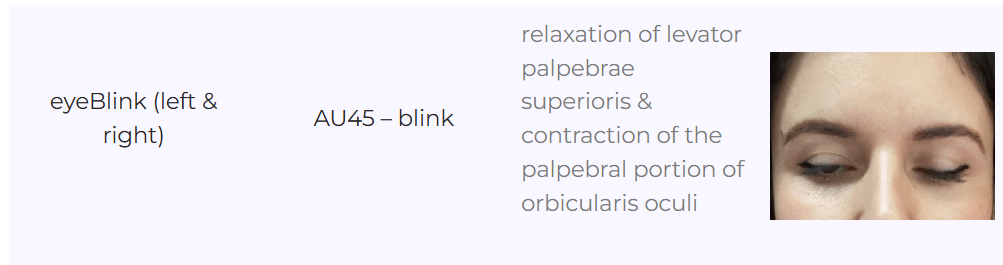
\includegraphics[width=0.95\linewidth]{figures/Fig_AUSample.png}
\caption{示例图来自~\cite{ozel_arkit_facs_cheatsheet},展示 FACS AU45(blink)对应的 ARKit 中的两种 BlendShape 基形:\texttt{eyeBlinkLeft}(闭左眼)与 \texttt{eyeBlinkRight}(闭右眼)。}
\label{fig:au_sample}
\end{figure}

图~\ref{fig:bs_eyeblink} 展示了 \texttt{eyeBlinkLeft}、\texttt{eyeBlinkRight} 基形在权重 $w\!\in\![0,1]$ 下的线性插值效果(从张眼到闭眼)。这使得 BlendShape 向量既便于作为可学习输入,又可直接映射到渲染引擎的驱动接口。

\begin{figure}[h!t]
\centering
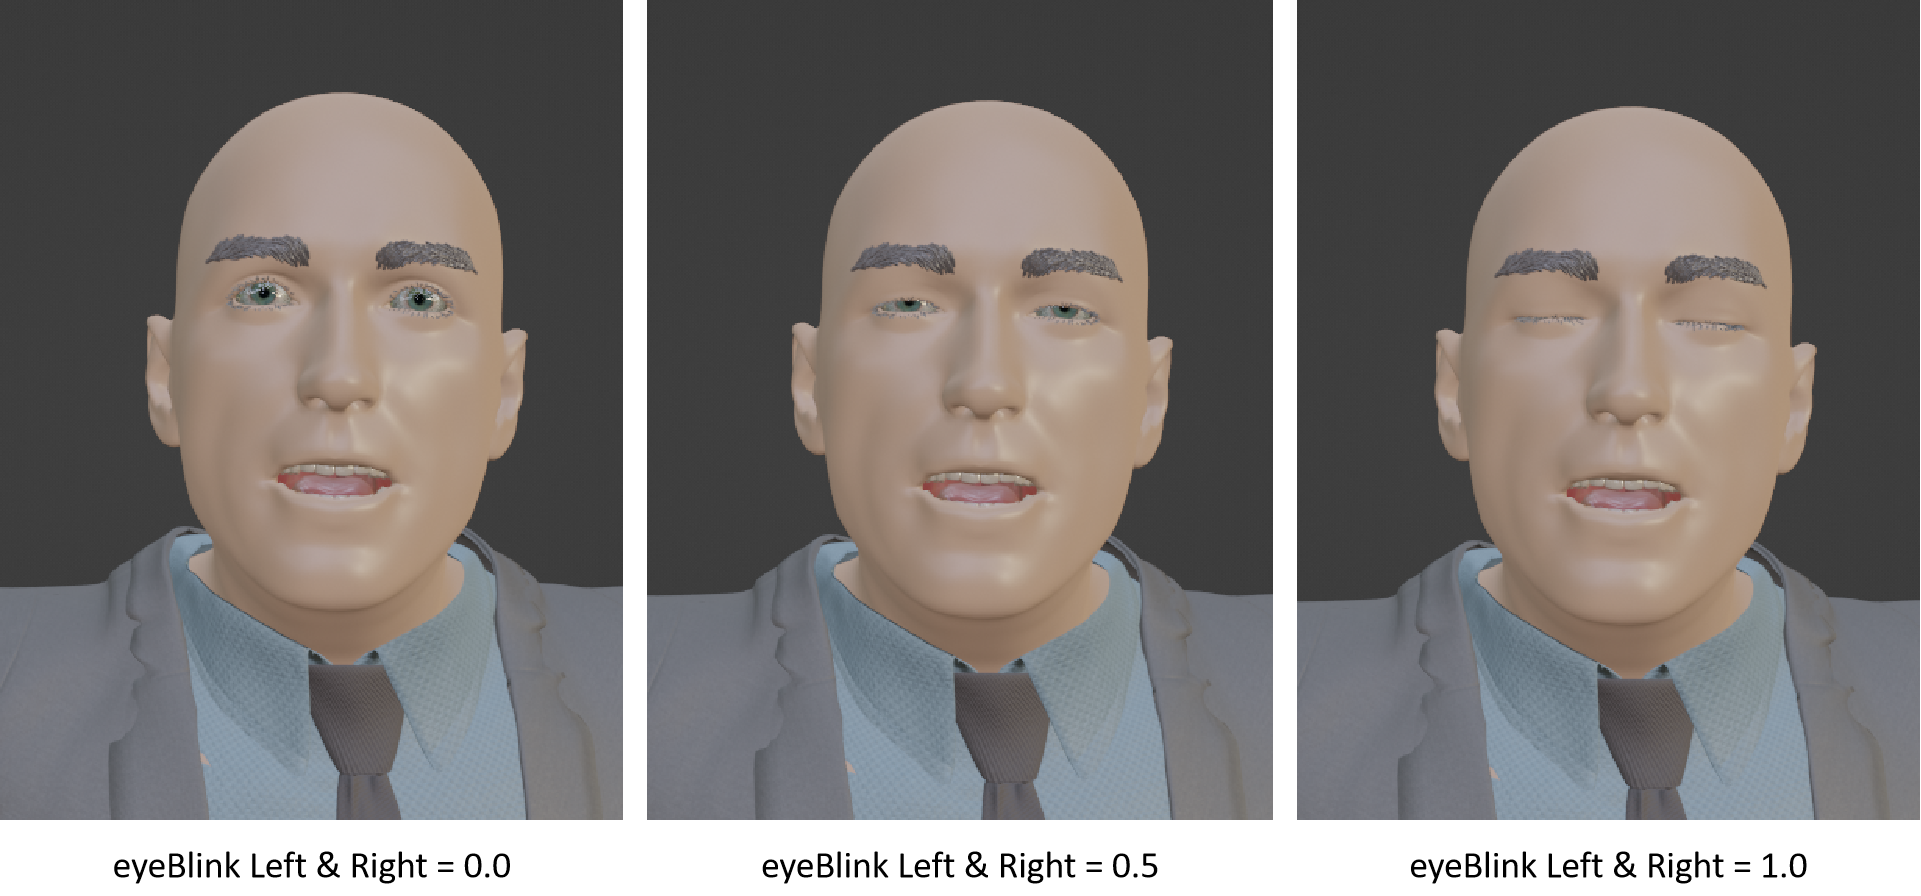
\includegraphics[width=0.95\linewidth]{figures/Fig_blendshapeEyeBlink.png}
\caption{BlendShape 线性插值效果示例:\texttt{eyeBlink} 从 $w{=}0$(左)到 $w{=}1$(右)的连续变化,中图为中间值。BS 权重可直接用于实时渲染驱动。}
\label{fig:bs_eyeblink}
\end{figure}

在具有相同网格结构的角色模型之间,BlendShape 基形集合可以直接复用,但在拓扑不同的模型间则需重新定义。

\paragraph{关键点坐标模型(Landmark-based Representation)}
关键点模型通过检测面部若干语义特征点(2D 或 3D 坐标)来描述几何结构变化。典型实现包括 MediaPipe Face Mesh \cite{mediapipefacemesh} 与 OpenFace 系列。

与基于网格形变的 BlendShape 不同,关键点模型并不依附于任何具体网格拓扑,而是在几何空间中以语义一致的特征点集合形式定义面部结构。这种表示方式并不描述模型的形变,而是对“人脸几何”的抽象建模,因此常用于表情识别、头部姿态估计等分析任务,而较少用于驱动渲染。

在多模态学习与特征分析中,BlendShape 表示具有较高的统一性和可量化性,适合以固定维度向量作为模型输入,并易于应用于不同虚拟角色的动画驱动。因此,本文在系统设计中采用与 ARKit 兼容的 BlendShape 参数作为面部模态输入特征。

\begin{figure}[h!t]
\centering
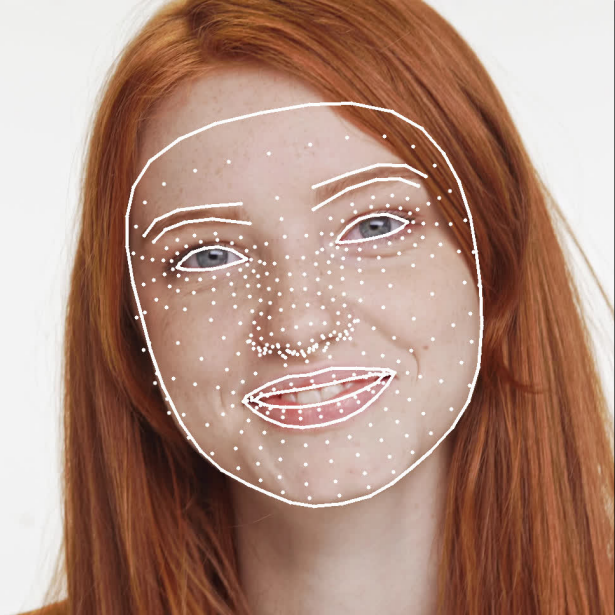
\includegraphics[width=0.4\linewidth]{figures/Fig_MediaPipeLandmark.png}
\caption{MediaPipe Face Mesh 关键点结构示意图,截取自 \cite{mediapipefacemesh}。}
\label{fig_mediapipe_landmark}
\end{figure}

\section{国内外研究现状}

\subsection{手势生成的研究目标}

\subsubsection{研究目标类型的差异}

语音驱动的手势生成研究在总体目标上虽一致——即让虚拟角色的动作与语音内容、节奏协调一致——但在使用场景与系统角色上存在显著差异。

现有研究大体可分为两类:

\paragraph{为AI的虚拟形象生成手势}

这一类研究的目标是让AI驱动的文本对话系统的虚拟形象具备手势表现力。

模型可以一次性生成下一句语音或文本,因此可以访问完整的未来信息,包括整句音频、文本和语义上下文。

典型方法通过编码完整句子的节奏与语义,预测整段动作轨迹,以最大化动作与语义的一致性和整体流畅性。

这类方法适合AI驱动的系统或离线生成的应用场景,如合成视频。

\paragraph{为用户的虚拟人生成实时手势}
本文所聚焦的目标类型属于第二类。

在用户实时说话的过程中,系统需根据当前语音流(以及可选的面部与头部模态)即时生成同步手势。

此任务具有严格的实时性约束与因果性限制:模型在每一时刻只能使用当前及过去的信息,而不能访问未来语音或文本内容。

因此,常见的整句式规划或滑动预测方法不再适用。

该任务更接近实时交互系统,而非内容生成系统。

\subsubsection{任务约束与可利用条件的差异}

这两类研究目标在可利用的信息条件和评价重心上存在本质区别:

\begin{table}[h]
\centering
\caption{两类手势生成任务在约束与可利用条件上的对比}
\label{tab:task_constraint_comparison}
\begin{tabular}{@{}p{3cm}p{5.5cm}p{5.5cm}@{}}
\toprule
\textbf{对比维度} & \textbf{AI 虚拟形象生成} & \textbf{用户虚拟人实时生成} \\ 
\midrule
输入信息 & 完整句级语音或文本(可使用未来信息) & 实时语音流,仅使用过去与当前帧 \\ 
输出目标 & 整句手势序列(离线生成) & 连续流式手势(逐帧生成) \\ 
时间约束 & 不必要实时 & 帧级实时性($<$50\,ms 推理延迟) \\ 
评价重点 & 整体语义一致性与美学自然度 & 瞬时同步性、动作平滑与交互稳定性 \\ 
应用场景 & 离线动画、内容合成、AI虚拟直播 & 实时虚拟人、视频会议、用户虚拟直播 \\ 
\midrule
语音模态 & 作为输入或由文本生成(TTS 输出) & 作为实时输入特征(语音流) \\ 
手部手势 & 生成目标(输出) & 生成目标(输出) \\ 
面部表情 & 通常为生成目标(输出) & 可通过设备实时采集,作为输入辅助推理 \\ 
头部姿态 & 通常为生成目标(输出) & 可实时采集并作为输入特征,用于同步推理 \\ 
\bottomrule
\end{tabular}
\end{table}

前者可以在生成阶段规划动作节奏与语义对应,而后者需在无未来信息的条件下维持自然与同步,
并保证输出连续、平滑且无突跳,从而对模型结构、输入模态与延迟控制提出更高要求。

\subsubsection{评估方法}

语音驱动手势生成研究的评价体系通常涵盖生成质量、时序匹配与表达多样性等多个维度。
研究者既关注生成动作的自然性与视觉流畅度,也重视其与语音信号在节奏和语义层面的对应关系。
近年来,随着实时生成和多模态扩展任务的发展,相关评估方法也逐渐体系化,可概括为以下几类:

\begin{enumerate}
    \item \textbf{自然性(Naturalness)} —— 衡量生成动作在运动平滑性、速度变化及能量分布上的合理性,常采用 FGD(Fréchet Gesture Distance)\cite{ginosar2019speech2gesture}、
          运动速度统计、或主观“自然度”评分等指标。
    \item \textbf{同步性(Synchronization)} —— 评估手势在时间上与语音重音或韵律事件的对齐程度,
          常用 BA(Beat Alignment)\cite{kucherenko2021predictability}、DTW(Dynamic Time Warping)等方法,
          以及基于重读检测的主观同步性评价。
    \item \textbf{多样性(Diversity)} —— 衡量模型在不同语音输入下生成的动作变化程度,
          通常以轨迹分布的方差、速度曲线差异或 L1DIV 等指标度量,
          以防止模型陷入单一模式或过度平滑。
    \item \textbf{语义相关性(Semantic Relevance)} —— 反映生成动作与语义关键词或情绪类别的一致性,
          可通过 SRGR(Semantic Relevance to Gesture Ratio)\cite{beatcamn} 等指标或人工标注语义标签对齐评估。
    \item \textbf{实时性与稳定性(Latency \& Robustness)} —— 在面向交互系统的研究中,
          还需评估帧级推理延迟与输出平滑性,以确保动作流连续且系统响应及时。
\end{enumerate}

总体而言,现有评价体系既包含客观的运动学与统计指标,也结合主观感知评分,
在不同任务目标下可形成“自然性—同步性—多样性—相关性”的综合评估框架。

\subsection{手势生成的演变}

近年来,语音驱动手势生成经历了从规则设计到数据驱动模型、再到多模态扩展与实时生成的持续演变。
这一过程不仅体现了算法架构的更新,也反映了研究目标与应用场景的变化:
从基于语言规则的行为映射,到学习语音—动作关系的深度生成模型,再到面向交互的多模态实时系统。

\subsubsection{规则驱动阶段}

早期的手势生成系统主要依赖语言学规则与专家知识构建 \cite{behavior_expression_animation_toolkit,robot_behavior_toolkit,gesture_generation_by_imitation,gesture_and_speech_in_interaction}。
这类方法通过语义分类或韵律规则将语音片段映射为预定义的手势模板(如指示、肯定、节奏性动作),并以有限的动作库组合出手势序列。
典型代表如 BEAT toolkit 与 Robot Behavior Toolkit,它们可在虚拟代理或机器人中实现基于语音的同步动作。
然而,手势词典与语法规则的人工设计成本较高,难以覆盖自然语音中的多样变化,导致生成结果缺乏自然性与个体差异。

\subsubsection{数据驱动阶段}

随着大规模语音与动作配对数据的出现,研究者开始采用统计学习和深度神经网络模型学习语音—手势映射关系。
在此阶段,语音通常作为唯一输入模态,模型通过 LSTM、GRU 或 MLP 等结构预测连续手势序列。
典型代表如 CaMN 模型 \cite{beatcamn},其基于 BEAT 数据集 \cite{beatcamn} 训练级联网络,将 LSTM、全连接网络与 GAN 结构相结合,实现从语音到动作的端到端预测。

然而,该类模型多使用欧拉角或离散旋转参数作为手势表示,生成结果容易出现抖动与不连续。
后续工作引入更平滑的表示方式,如 Rot6d \cite{rot6d,emage,AMUSE2024} 或 Axis-Angle \cite{diffsheg},显著提升了动作流畅性。
与此同时,为解决语音与手势间的多对多映射问题,研究者引入了 VQ-VAE \cite{emage,zhang2024SemanticGesticulator} 与扩散模型 \cite{tamingDiffgesture,diffsheg,diffstylegesture,DiffTED2024,diffusion-self-supervised2023},
在保持自然性的同时提升了生成多样性与表现力。

尽管这些方法在客观指标与视觉效果上均优于传统模型,但它们普遍假设可访问完整语音或文本上下文,
属于“整句式(non-streaming)”生成,推理延迟较高,不适用于实时应用。
即便是推理效率较高的模型(如 CaMN、DiffSHEG),也因上下文缓冲机制而引入明显延迟。

\subsubsection{多模态扩展阶段}

为进一步提升动作表现力与语音理解能力,部分研究引入视觉模态或语言语义特征。
例如,CaMN \cite{beatcamn} 在语音输入的基础上融合面部捕捉信息以增强表现;
EMAGE \cite{emage} 与 DiffSHEG \cite{diffsheg} 同时生成手势与面部动作;
DiffTED \cite{DiffTED2024} 更进一步,实现了端到端的视频合成,使虚拟角色的语音、面部与肢体同步生成。

这些多模态生成方法在提升虚拟智能体的自然感与沉浸感方面表现优异,但其任务假设仍基于整句输入,因此主要用于AI 虚拟形象生成或离线内容创作场景,而非实时用户交互。

\subsection{当代生成研究的策略趋势}
尽管 McNeill 的分类提供了语义层面的参考,但实际的手势生成任务常针对可观测与可学习的特征进行抽象。近年的研究在数据建模层面主要呈现三种策略:

\begin{enumerate}
  \item \textbf{简化标签法(Simplified labeling)}:为降低多部位、多语义类别手势的标注与分类难度,
    研究者通常将所有身体层动作(包括手部与头部)统一划分为
    “节奏型(beat-like)”与“语义型(semantic-like)”两大类,
    而不再严格遵循 McNeill 针对手部动作的四类划分。
    这种方式在语音—动作对齐任务中更具可操作性,
    特别适用于以韵律为核心驱动的生成模型。
    由于节奏型(beat-like)手势与头部动作均与语音韵律的时间结构高度耦合,
    现有研究往往采用此简化策略,即不对数据集进行显式语义类别标注,
    而仅通过语音—动作对齐学习可观测的节奏模式。
    这种策略可视为“弱标签化(weakly-labeled)”的实现形式,能够避免语义标注成本,并在实时生成任务中取得稳定的同步效果。
  \item \textbf{语义增强方向(Semantic-aware generation)}:部分工作尝试通过语义或文本特征扩展生成范围,以覆盖 \emph{iconic} 或 \emph{metaphoric} 手势。例如 Yoon 等(2020)\cite{yoon2020speechgesturebert} 将语音与文本嵌入结合;Alexanderson 等(2023)\cite{alexanderson2023diffgesture}引入上下文风格控制,实现了语义相关的动作变化。
  \item \textbf{混合式生成策略(Hybrid generation)}:以数据驱动的节奏型(beat-like)底流确保全时连续与韵律对齐,在检测到关键语义事件时,通过规则/检索/模板短片段进行语义强化,并在边界处通过速度与加速度匹配实现无缝过渡。该思路得到近期综述与语义检索式系统的支持\cite{zhang2024SemanticGesticulator},同时 BEAT 数据集提供的语义相关性标签可直接作为触发信号\cite{beatcamn},便于工程化落地。与纯数据驱动的扩散式手势生成\cite{alexanderson2023diffgesture,tamingDiffgesture}以及实时多模态生成\cite{diffsheg}相比,混合式能够在不牺牲节奏自然度的前提下,增强语义显著时刻的表达力。
\end{enumerate}

\section{实时生成的理论基础与可行性分析}
从生成可行性的角度,现有研究普遍认为 \emph{beat} 手势可在无语义理解的条件下由语音韵律直接驱动生成。
大量语音驱动手势研究证实,仅凭语音的能量、时长与音高变化即可合成自然的节奏性上肢动作\cite{ginosar2019speech2gesture,alexanderson2020stylegestures,kucherenko2021movingfastslow}。
这些研究所生成的动作在时间结构上与语音重音同步,体现了语音与手势共享的时间规划机制。

相比之下,\emph{iconic}(形象性)、\emph{metaphoric}(隐喻性)与 \emph{deictic}(指向性)手势均依赖语义或指向关系,需要对话语境或文本语义输入,
难以在严格实时的因果条件下生成。Kucherenko 等\cite{kucherenko2021predictability} 的可预测性分析进一步验证了这一点:
他们发现手势的语义类别和空间指向性在语音特征中几乎不可预测,即便结合文本特征,预测性能也相当有限,
而节奏阶段(phase)相关特征在音频中则具有显著更高的可预测性。
这表明,在缺乏未来语义与全局上下文的实时场景中,仅凭语音模态,模型只能稳定生成节奏层面的动作。

然而,本文的研究在此基础上进一步引入了\emph{头部姿态模态}作为补充输入信号。
与手部动作相比,头部姿态能直接反映注意、指向和互动焦点等空间要素。
因此,虽然 \emph{deictic} 手势在语音和文本模态中难以预测,
但结合头部姿态输入后,模型可以部分恢复空间指向性信息,
在实时约束下生成具有方向感与互动特征的动作成为可能。
这一点构成了本文模型设计的重要理论依据。

\paragraph{头部姿态模态的建模意义}
头部姿态模态不仅与语音韵律在时序上高度耦合,
还能提供语义与情感层面的补充信号。
其不同类型的头部手势——包括韵律型、语义/态度型、指向型与预测型——
在建模上分别发挥以下作用:
\begin{enumerate}
  \item \textbf{韵律同步:}头部动作与语音重音、句法节奏具有高时间一致性,
        其速度与幅度变化可作为语音能量、时长与重读的外显指标,
        有助于模型捕捉语音节奏结构并增强手势的时间同步性;
  \item \textbf{情绪反馈:}头部的肯定、否定或强调动作提供即时的情感线索,
        在语音语义模糊时帮助模型区分发话倾向与语气;
  \item \textbf{指向与注意:}转头与注视方向反映说话者的注意焦点,
        在时间上为手势触发提供“方向性约束”,
        可提升空间一致性与互动感;
  \item \textbf{预测信号:}微小的预点头或抬头动作往往早于声学重读出现,
        为模型提供时间上的“前瞻信号”,
        以弥补因果条件下缺乏未来语义信息的不足。
\end{enumerate}
从工程角度看,头部姿态输入既能在节奏层面补充韵律一致性,
又能在空间层面提升对话的自然交互感,
因此在实时语音驱动任务中成为极具价值的输入模态。

\paragraph{头部模态补充语音驱动的空间指向性预测}
如前所述,Kucherenko 等\cite{kucherenko2021predictability} 的研究表明,
手势的空间指向性在语音与文本模态中可预测性均较低,
这意味着传统纯语音驱动系统难以生成具有明确空间方向的动作。
然而,头部姿态模态天然携带了空间线索:
其转头与注视变化反映了注意目标与话题焦点,
而预测型点头可提前暗示节奏或发音峰值。
因此,在实时生成模型中,
引入头部模态不仅增强了韵律一致性,
更为生成具方向感的\emph{deictic}类手势提供了信息基础。

尽管如此,模型仍存在边界:
头部模态信号受设备噪声与说话风格差异影响,
难以完全替代语义理解或文本上下文。
因此,本文模型在设计上以 \emph{beat-like} 手势为基石,
保留对 \emph{deictic} 手势的有限触发能力,
而不追求生成 \emph{iconic} 与 \emph{metaphoric} 手势。
这种策略在保证实时性与稳定性的同时,
兼顾空间表达与自然度,为多模态实时生成提供了理论与实践的平衡点。

\section{本文的工作与创新点}

本文研究的目标是设计一种能够在实时条件下运行的语音驱动手势生成模型,使用户无需动作捕捉设备或特定硬件,仅通过语音输入即可驱动虚拟人的上肢与头部动作。与以往主要面向离线生成或 AI 虚拟形象生成的研究不同,本文关注的任务场景是“用户实时交互”,因此系统必须在严格因果的条件下运行,即只能利用当前与过去的输入帧信息,无法依赖未来语音或文本内容进行整体规划。

现有的高精度手势生成模型在离线场景中表现优异,特别是基于扩散模型或 VQ-VAE 的方法 \cite{tamingDiffgesture, diffsheg, emage, DiffTED2024}, 能够生成自然、连贯且语义相关的手势序列。然而,这些模型通常需要整句语音或文本作为输入,推理过程依赖未来信息以分析语义结构与节奏特征,  
因此难以直接应用于实时交互系统。在无未来信息约束下,模型必须在信息不完整的情况下进行预测,这会显著影响动作生成的自然性与语义一致性。

为缓解上述问题,本文提出利用用户的面部表情与头部姿态作为辅助输入模态,为手势生成过程提供额外的非语言信号。面部表情能反映说话者的情绪与语气变化,在语义模糊的情况下有助于生成更具情感表达的动作;头部姿态则能反映注意方向与交互焦点,在语音节奏变化时为手势生成提供时序上的参考。  
通过将这两种模态与语音信号联合输入模型,系统能够在实时条件下获得更多上下文线索,从而在保持低延迟的同时提升手势生成的自然度与一致性。

本文以 CaMN 模型 \cite{beatcamn} 为基础进行扩展。CaMN 原为离线级联结构,输入包括语音与面部捕捉特征,输出包含手部与头部姿态。本文首先将其输入机制改写为逐帧输入流形式,并引入新的头部特征分析模块,将头部姿态信号作为独立通道输入至级联网络的末端层,以强化模型的时序响应能力。  
在这一结构下,系统可在实时语音流输入条件下逐帧生成动作输出,实现语音、面部与头部信号的联合驱动。

实验结果表明,本文提出的模型在实时性与动作自然性之间取得良好平衡。在典型的桌面端环境下,单帧推理时间约为1毫秒之内,能够满足实时交互需求;同时在 FGD、BA 与主观评测中表现出与离线模型相近的手势自然度与同步性。由此,本文的方法证明了在严格因果条件下,通过多模态输入融合可以有效提升实时手势生成的表现力与稳定性。

\section{本章小结}
本章综述了语音驱动手势生成领域的相关研究现状与发展脉络。  
首先,对手势的概念与在计算机中的参数化表示进行了阐述,说明了手势与面部表情、头部姿态在虚拟人交互中的角色与差异。  
随后,从研究目标的角度分析了不同任务设定之间的区别,指出现有大多数工作聚焦于为 AI 虚拟形象生成整句级动作,而缺乏面向用户实时交互的研究。  
在此基础上,回顾了手势生成方法从规则驱动到数据驱动、从单模态到多模态的演变过程,  
总结了现有模型虽在生成质量上取得显著进展,但在实时性与因果性方面仍存在局限。

最后,结合本文的研究目标,提出了面向实时交互的语音驱动手势生成方案。


 % !TEX root = ../main.tex

\chapter{方法}

\section{研究定位与总体设计思路}
手势可根据语义依赖性与时间结构复杂度区分为可语义生成与可韵律生成两大类。
本文的研究聚焦于严格实时的语音驱动任务,在此条件下模型无法访问未来语音或完整语义,
因此重点生成与语音韵律同步的 \emph{beat-like} 手势及头部动作,
并通过面部与头部模态的联合输入进一步增强表达性与自然度。
这种选择既符合认知语言学的节奏—动作一致性原则,也符合实时系统的因果约束。

基于上述定位,本文提出了一种基于音频、面部 BlendShape 权重和头部姿态输入的
帧级多模态级联手势生成模型 \emph{FaceCapGes}。
模型旨在在实时条件下实现自然、同步且具有一定指向性的上半身动作生成,
在不依赖语义理解或未来上下文的前提下,
通过多模态输入弥补语音模态预测能力的不足。

为避免与系统级说明混淆,本文模型在第~\ref{sec:system}~节首先给出端到端系统定位;
随后在第~\ref{sec:problem}~节形式化定义任务与符号体系;
在第~\ref{sec:cascade}~节详细阐述模型的级联结构与输入模态设计;
最后在第~\ref{sec:training}~节说明训练过程与优化方法;
并在第~\ref{sec:implementation}~节介绍实现细节与训练配置。

\section{系统整体框架与模块定位}
\label{sec:system}
本节介绍整个系统的端到端驱动流程及模块职责划分。如图~\ref{fig:system_architecture} 所示,系统整体架构由五个层级组成:用户配置层、设备层、中间件层、手势生成模型层以及渲染与驱动层。各层之间通过多模态信号接口进行连接,实现从信号采集到虚拟人动作生成的端到端实时处理。

FaceCapGes 模型位于中间层,承担多模态输入到上半身姿态输出的核心推理任务,而输入采集与渲染模块分别负责信号获取与结果展示。

为实现基于语音、面部捕捉与头部姿态的实时数字人驱动系统,本文构建了完整的信号采集、动作生成与渲染展示的处理管线。FaceCapGes 模型作为该系统的核心计算模块,负责在实时约束下从多模态输入推理出当前帧的上半身骨骼姿态。

\begin{figure*}[h!t]
\centering
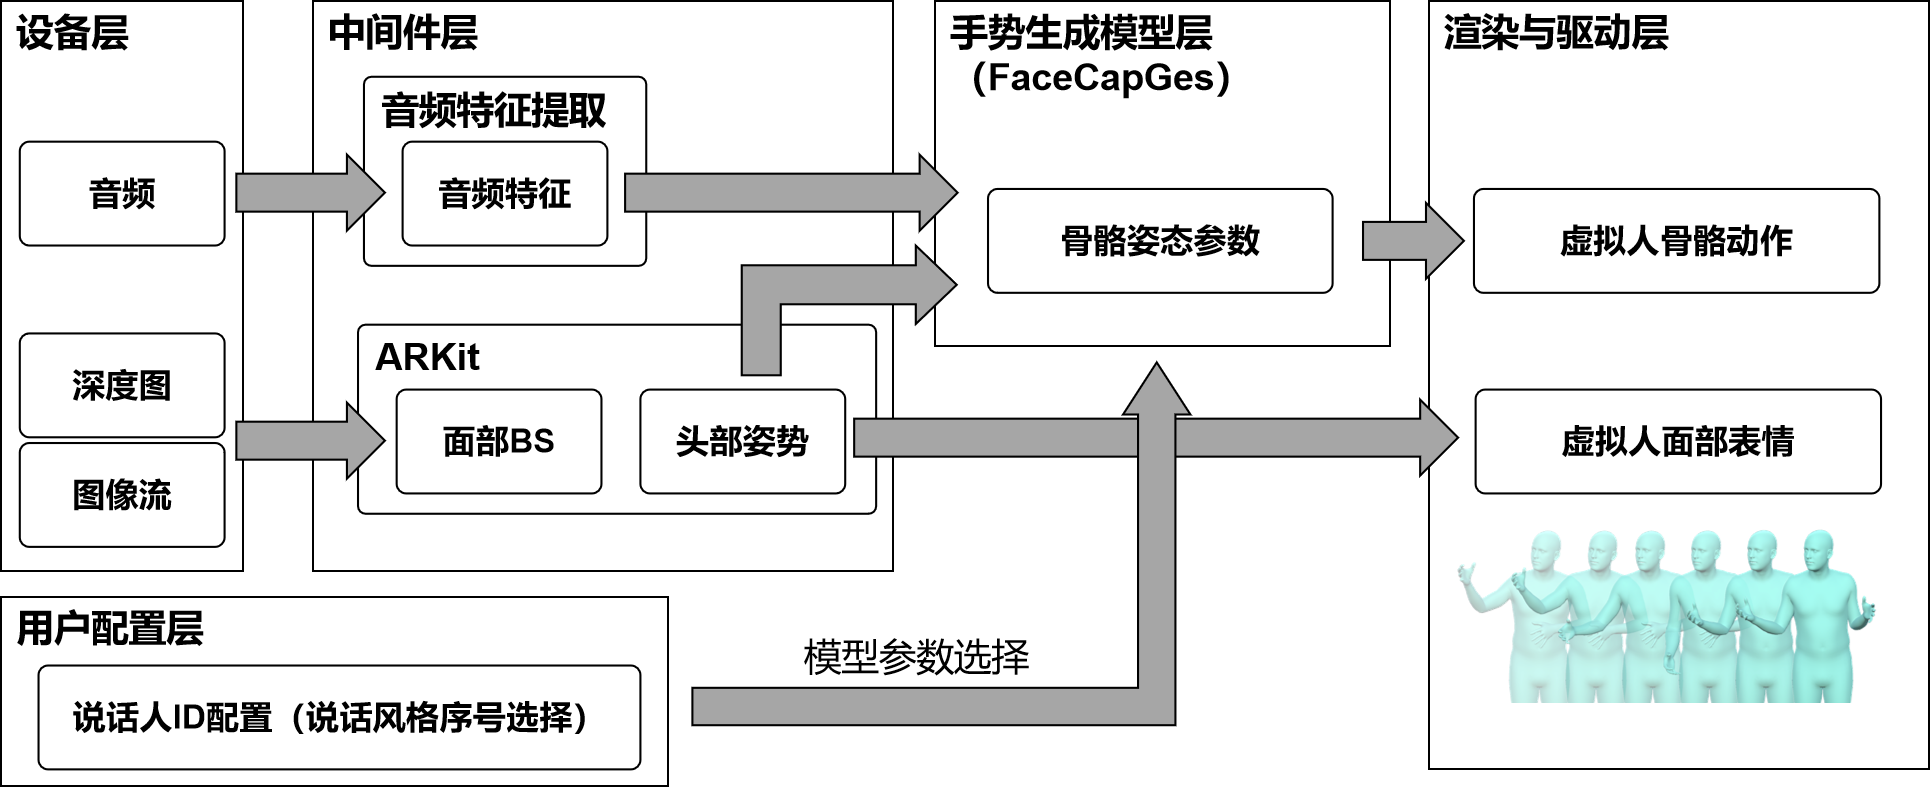
\includegraphics[width=\textwidth]{figures/SystemArchitecture.png}
\caption{系统整体架构与数据流示意图}
\label{fig:system_architecture}
\end{figure*}

\subsection{信号采集与系统配置层}
该层位于系统整体架构的输入端,用于从用户端设备实时获取多模态信号,并在系统初始化阶段完成运行参数的配置。整体结构可划分为设备层、中间件层与用户配置层三个部分,如图~\ref{fig:system_architecture} 所示。

\paragraph{设备层}
设备层负责采集语音与视觉模态信号。语音信号由麦克风实时录制,采样率与帧移可根据运行设备性能调整;视觉信号由前置 TrueDepth 摄像头获取面部深度图与视频流,并作为 ARKit 面部追踪模块的输入。

\paragraph{中间件层}
中间件层通过 Apple 提供的 ARKit 框架,将设备层的原始图像流与深度图转化为结构化特征。ARKit 输出两类主要数据:  
(1) \textbf{面部表情特征} ARKit 提供 52 维 BlendShape 系数向量,用于描述关键肌肉群的局部形变状态。该特征能够反映用户的表情、口型与情感变化,并以帧级形式同步输出。  
(2) \textbf{头部姿态特征} ARKit 在 ARFaceAnchor 对象中输出一个 $4\times4$ 齐次变换矩阵 $\mathbf{T}=[\mathbf{R}|\mathbf{t}]$,其中左上角的 $\mathbf{R}\in\mathbb{R}^{3\times3}$ 为旋转矩阵,右上角的 $\mathbf{t}\in\mathbb{R}^{3\times1}$ 为平移向量。本研究从矩阵中提取旋转部分,并将其转换为Rot6D\cite{rot6d}表示形式,以提升旋转空间的连续性与模型训练的稳定性。  

同时,音频流在中间件层中被传入特征提取模块以生成时间序列特征。模型训练阶段使用 Librosa 库离线提取 Mel 频谱、短时能量(RMS)与基频 $F_0$ 等声学特征,以保证特征精度与一致性。系统运行阶段可由等价的实时特征提取模块(如 torchaudio 或 TensorFlow Audio)逐帧生成对应特征,以实现端到端的低延迟运行。

\paragraph{用户配置层}
用户配置层负责系统初始化阶段的模型与参数设定。用户可在应用中选择说话风格,对应加载不同说话人ID配置下的模型权重。该配置仅在系统启动时生效,不参与实时推理过程。

本层提供的多模态信号经中间件处理后,以统一的数据接口传递至手势生成模型,实现语音、表情与头部姿态的实时融合输入。

\subsection{手势生成模型层(FaceCapGes)}

FaceCapGes 模块位于系统的中间层,是本文提出的核心计算单元。该模块接收来自信号采集与系统配置层的三类输入特征:语音特征、面部 BlendShape 系数以及头部姿态参数,并在不依赖未来帧的条件下,逐帧预测用户当前时刻的上半身骨骼姿态。

生成的骨骼姿态采用 Rot6D 连续旋转表示形式,覆盖上半身 47 个关节的旋转参数。模型内部通过级联多模态编码结构提取时序相关特征,并利用单向 LSTM 解码器完成时间依赖建模,从而在保持实时性的同时,生成与语音节奏、表情变化及头部朝向高度一致的自然手势。

FaceCapGes 输出的姿态数据通过统一接口传递至渲染与驱动模块,与实时面部捕捉信号共同驱动虚拟角色的整体动作。由于模型仅依赖当前与历史帧输入,可与输入层以固定帧率并行运行,实现端到端的低延迟推理。

\subsection{渲染驱动层}

该模块位于系统输出端,负责将手势生成模型与面部捕捉结果共同转化为虚拟人的实时动作表现。
系统将 FaceCapGes 模型输出的上半身骨骼姿态与 ARKit 实时生成的 52 维面部 BlendShape 系数传递至渲染引擎,
由引擎内编写的脚本模块解析并映射至目标虚拟人的骨骼与表情控制接口,从而实现多模态动作驱动。

渲染模块采用基于 GPU 的蒙皮计算与实时光照模型,以确保动画的平滑性和视觉一致性。
最终,系统能够在实时流式输入条件下稳定运行,
同步呈现语音、表情与身体动作,
以自然流畅的数字人形象实现从多模态信号输入到可视化输出的完整驱动流程。

\section{问题定义}
\label{sec:problem}

在整体系统中,FaceCapGes 模块承担着从多模态输入信号到上半身骨骼姿态预测的核心任务。
为了明确模型的输入输出结构与学习目标,本节对该问题进行形式化定义。

\subsection{任务描述}

目标是在实时条件下,根据用户当前时刻的语音、面部表情与头部姿态信息,预测其对应的上半身骨骼姿态。模型需能够逐帧生成与语音节奏、面部动态和头部转动方向相协调的自然手势动作,而不依赖未来的输入帧或整句语音信息。

形式上,可以将该任务定义为一个多模态时序映射函数:
\begin{equation}
\hat{\bm{v}}_{t}^{B} = f_\theta\!\big(\bm{v}_{t-N:t}^{A},\, \bm{v}_{t-N:t}^{F},\, \bm{v}_{t-N:t}^{H}\big),
\end{equation}
其中 $f_\theta$ 表示由参数 $\theta$ 控制的预测模型,$N$ 为历史窗口长度。
%
各模态输入定义如下:
$\bm{v}_{t}^{A}$ 表示语音模态在时刻 $t$ 的特征向量,由麦克风信号经特征提取模块得到;
$\bm{v}_{t}^{F}$ 表示面部模态的输入,为 ARKit 输出的 52 维标准化 BlendShape 系数;
$\bm{v}_{t}^{H}$ 表示头部模态的输入,为 ARKit 得出的头部旋转矩阵经 Rot6D 表示;
而 $\hat{\bm{v}}_{t}^{B}$ 为模型在当前时刻预测的上半身骨骼姿态向量。
%
模型仅利用当前及过去 $N$ 帧的输入信息估计 $\hat{\bm{v}}_{t}^{B}$,
从而满足严格的实时推理约束。

\subsection{输入与输出模态}

FaceCapGes 模型的输入由三种可同时实时获取的模态组成:语音特征、面部 BlendShape 权重及头部姿态参数;输出为当前帧的上半身骨骼旋转状态。各模态的符号与维度如表~\ref{tab:modalities} 所示。

\begin{table}[h]
\centering
\caption{输入输出模态符号与维度}
\label{tab:modalities}
\begin{tabular}{llll}
\toprule
\textbf{模态} & \textbf{符号} & \textbf{维度} & \textbf{描述} \\
\midrule
语音特征 & $\bm{v}_t^{A}$ & $\mathbb{R}^{1067}$ & 由音频信号提取的时序特征(Mel 频谱、能量、基频等) \\
面部 BlendShape & $\bm{v}_t^{F}$ & $\mathbb{R}^{52}$ & ARKit 输出的标准化表情权重向量 \\
头部姿态 & $\bm{v}_t^{H}$ & $\mathbb{R}^{6}$ & 采用 Rot6d 表示的头部旋转参数 \\
骨骼姿态(输出) & $\hat{\bm{v}}_t^{B}$ & $\mathbb{R}^{6 \times 47}$ & 上半身 47 个关节的旋转状态 \\
\bottomrule
\end{tabular}
\end{table}

输入序列 $\big(\bm{v}_{t-N:t}^{A},\, \bm{v}_{t-N:t}^{F},\, \bm{v}_{t-N:t}^{H}\big)$ 描述了用户在过去 $N$ 帧内的语音与表情动态信息。模型通过学习其时序变化规律,逐帧生成对应的骨骼姿态输出 $\hat{\bm{v}}_t^{B}$。在推理阶段,模型仅访问至时刻 $t$ 的输入序列,无法访问任何未来帧信息,保证了生成过程的因果性与实时性。

\subsection{学习目标与优化形式}

在训练阶段,给定来自多模态语音动作数据集(如 BEAT)的配对样本:
\begin{equation}
\big(\bm{v}_t^{A},\, \bm{v}_t^{F},\, \bm{v}_t^{H},\, \bm{v}_t^{B}\big)
\end{equation}
模型的学习目标是最小化预测姿态 $\hat{\bm{v}}_t^{B}$ 与真实姿态 $\bm{v}_t^{B}$ 之间的差异。
综合考虑空间重构误差与时序平滑性约束,总体优化目标可表示为:
\begin{equation}
\mathcal{L}_{total} =
\mathcal{L}_{rec} + \lambda_v \mathcal{L}_{vel} + \lambda_a \mathcal{L}_{acc} + \lambda_{adv} \mathcal{L}_{adv}
\end{equation}
其中:
\begin{itemize}
    \item $\mathcal{L}_{rec}$ 为姿态重构损失,衡量单帧旋转角度误差;
    \item $\mathcal{L}_{vel}$、$\mathcal{L}_{acc}$ 分别约束预测序列的速度与加速度连续性;
    \item $\mathcal{L}_{adv}$ 为对抗损失,用于提升生成手势的自然性;
    \item $\lambda_v, \lambda_a, \lambda_{adv}$ 为对应的权重系数。
\end{itemize}

通过最小化上述综合损失,模型能够在不依赖未来帧的条件下生成自然、流畅且与语音节奏相匹配的上半身动作序列。

\section{级联架构与输入模态设计}
\label{sec:cascade}

\subsection{级联架构的原理与理论背景}

现有语音驱动手势生成模型多采用多模态融合结构,其中以 CaMN \cite{beatcamn} 为代表的级联架构在设计理念上具有代表性。其核心思想是将语音、面部表情与身体动作视为语义表达的不同层级:语音模态承担语义与节奏驱动作用,面部模态反映情感与意图,身体动作则是语言与情绪的外化呈现。CaMN 采用自上而下的处理顺序,即依次对语音、面部和动作模态进行建模,从而以层次化结构保持模态间的语义依存关系。

这种设计符合人类交流中“语言、表情、动作”一体化的认知规律\cite{mcneill_1992_hand, kendon_2004_gesture}。语音先规划语义与节奏,面部表情作为情绪强化信号随后产生,最终通过身体动作完成完整的非语言表达。模型中,语音编码器输出的时间嵌入被输入至面部编码器,再与面部特征融合后驱动动作解码器,从而保持语义一致性并增强表现力。

然而,CaMN 的原始设计面向离线整句生成任务,需要访问未来上下文以维持全局连贯性。在实时场景下,这种依赖将引入显著延迟并破坏因果性。FaceCapGes 在继承其层次思想的同时,对输入模式、训练方式与模态选择进行了系统性重构,以满足帧级实时约束。

\subsection{基线模态继承与实时适配}
FaceCapGes 保留了 CaMN 的语音与面部模态结构,但针对实时生成任务进行了适配性改写。

\subsubsection{说话人 ID 分支移除}
如图~\ref{fig:system_architecture}所示,用户配置层会设置说话人ID配置用于模型切换,但该模态在本模型中不属于网络输入。
在基线模型 CaMN 中,输入模态包含显式的说话人 ID 向量,用于在同一模型内区分不同演讲者的风格差异。
然而在实时交互场景下,该分支并非必要:用户身份通常固定,且说话风格的变化频率远低于帧级推理速度。
因此,FaceCapGes 移除了 ID 输入分支,并采用“单说话人训练”策略,即针对每个说话人独立训练模型参数。
实验表明,该方式能在保持收敛稳定的同时显著提升动作的自然性与节奏一致性。
从系统使用角度看,不同模型可视为“说话风格配置文件”,用户仅在需要时切换对应参数,该操作发生频率低,不会影响实时推理性能。

\subsubsection{输入模态继承}

语音特征通过时间卷积网络(Temporal Convolutional Network, TCN)和多层感知机(MLP)编码,以捕捉短时节奏模式;面部模态采用相似结构,并在中间层融合语音嵌入,从而增强语音与表情之间的语义关联。  
语音编码器 $E_A$ 与面部编码器 $E_F$ 的输出定义为:
\begin{equation}
\bm{z}^{A}_t = E_A(\bm{v}_{t-N:t}^{A}), \quad
\bm{z}^{F}_t = E_F(\bm{v}_{t-N:t}^{F};\, \bm{z}^{A}_t)
\end{equation}
其中 $\bm{z}^{A}_t \in \mathbb{R}^{128}$,$\bm{z}^{F}_t  \in \mathbb{R}^{32}$。
这两个编码器负责提取低层次语音节奏与表情动态信息,为后续模态融合提供稳定上下文表征。

此外,系统在此基础上引入头部姿态模态 $\bm{v}_t^{H}$,用于补充空间方向与节奏信号。
其编码器 $E_H$ 将 Rot6D 表示的头部旋转向量映射为紧凑潜在表征:
\begin{equation}
\bm{z}^{H}_t = E_H(\bm{v}_{t-N:t}^{H}),
\end{equation}
编码器结构将在第~\ref{sec:head_encoder}~节详细说明。

\subsubsection{输出模态继承(身体姿态解码)}

在输入模态经过编码与融合后,模型需将多模态特征映射至对应的身体姿态空间。
为实现层次化的动作生成与结构协调,本文将上半身的输出区域划分为两个互补分支:
躯干 (Torso, T)与上肢 (Upper limbs, U)。
躯干部分包含脊椎的三个主要控制关节,用于确定身体的姿态基准与运动节奏;
上肢部分包含双臂及手部关节,负责生成与语音节奏及情绪表达相呼应的细节动作。
最终的上半身姿态表示为两者的组合:
\begin{equation}
\bm{v}^B = \bm{v}^T \otimes \bm{v}^U,
\end{equation}
其中 $\otimes$ 表示通道维度拼接操作。

该分层设计继承了 CaMN 的层次预测思路:
模型首先生成相对稳定的躯干姿态以确定整体方向,
再以此为条件预测上肢动作,从而在实时生成中保持整体协调性与自然度。

具体而言,来自语音、面部与头部编码器的特征
$\bm{z}_i^{A}$、$\bm{z}_i^{F}$、$\bm{z}_i^{H}$ 会与历史姿态序列 $(\bm{v}_{i-N}^{B}, \ldots, \bm{v}_i^{B})$ 拼接,组成多模态隐向量:
\begin{equation}
\bm{z}_i^{M} = \bm{z}_i^{A} \otimes \bm{z}_i^{F} \otimes \bm{z}_i^{H} \otimes (\bm{v}_{i-N}^{B}, \ldots, \bm{v}_i^{B}),
\end{equation}
其中 $\otimes$ 表示通道维度拼接操作,时间末帧采用零填充以对齐维度。

随后,$\{\bm{z}_0^{M}, \ldots, \bm{z}_N^{M}\}$ 经两个单向 LSTM 解码器,分别生成躯干与上肢的潜在特征:
\begin{equation}
\bm{z}^{T} = \mathrm{LSTM}_{T}(\bm{z}_0^{M}, \ldots, \bm{z}_N^{M}), \quad
\bm{z}^{U} = \mathrm{LSTM}_{U}(\bm{z}_0^{M}, \ldots, \bm{z}_N^{M}),
\end{equation}
并通过独立的 MLP 模块还原为旋转参数:
\begin{equation}
\hat{\bm{v}}^{T} = \mathrm{MLP}_{T}(\bm{z}^{T}), \quad
\hat{\bm{v}}^{U} = \mathrm{MLP}_{U}(\bm{z}^{U}).
\end{equation}
最终拼接得到当前帧的完整上半身姿态:
\begin{equation}
\hat{\bm{v}}^{B} = \hat{\bm{v}}^{T} \otimes \hat{\bm{v}}^{U}.
\end{equation}

在推理阶段,解码器隐状态在时间步之间保持连续,
与前述输入模态特征配合,使模型在保持因果性的同时具备自然的时间平滑性。
由于该部分结构沿用自基线模型,本文不再赘述。
接下来,将介绍时间建模结构的改动及其对实时性的适配。

\subsubsection{时间建模结构改动与因果性约束}

基线模型 CaMN 使用双向 LSTM生成完整序列的骨骼姿态,输入与输出片段长度一致。
由于双向结构在每个时间步都依赖未来帧隐状态,虽然能增强整体平滑性,但不满足实时生成场景的因果约束。
为实现严格的实时性,本文将时间建模模块改为单向 LSTM,
使模型在每一时间步仅依赖过去 $N$ 帧的输入并预测当前帧的骨骼姿态。
虽然单向 LSTM 结构上仍会输出与输入片段等长的时间序列,但训练时仅计算其最后一帧的预测误差:

\begin{equation}
\hat{\bm{v}}_{t} = \mathrm{LSTM}(\bm{z}_{t-N:t}^{M})_{N}, \quad
\mathcal{L}_{\text{causal}} = \|\hat{\bm{v}}_t - \bm{v}_t\|_2^2,
\end{equation}

其中,下标 $N$ 表示取 LSTM 输出序列的最后一帧作为当前时刻的预测结果。

该策略通过在前 $N$ 帧内累积隐状态,于第 $N+1$ 帧完成当前姿态预测,从而建立严格的因果时序映射。

在推理阶段,FaceCapGes 采用长度为 $N$ 的显式输入窗口,并在时间步之间保留 LSTM 的隐状态。
虽然单向 LSTM 理论上能够仅通过递推隐状态存储历史信息,
但由于隐状态为压缩形式,难以完全保留短时节奏与相位特征。
因此,显式窗口输入与隐状态记忆在模型中形成互补:
前者提供局部的高分辨率上下文,
后者维持全局的时序连贯性。
这种设计在保证因果性的前提下提高了生成的稳定性与自然性,
也是实现实时语音驱动动作生成的关键因素之一。

图~\ref{fig_lstmcompare} 展示了双向与单向结构的差异:单向结构仅依赖历史帧输入,更适合在流式序列中逐帧输出预测结果。

\begin{figure}[h!t]
\centering
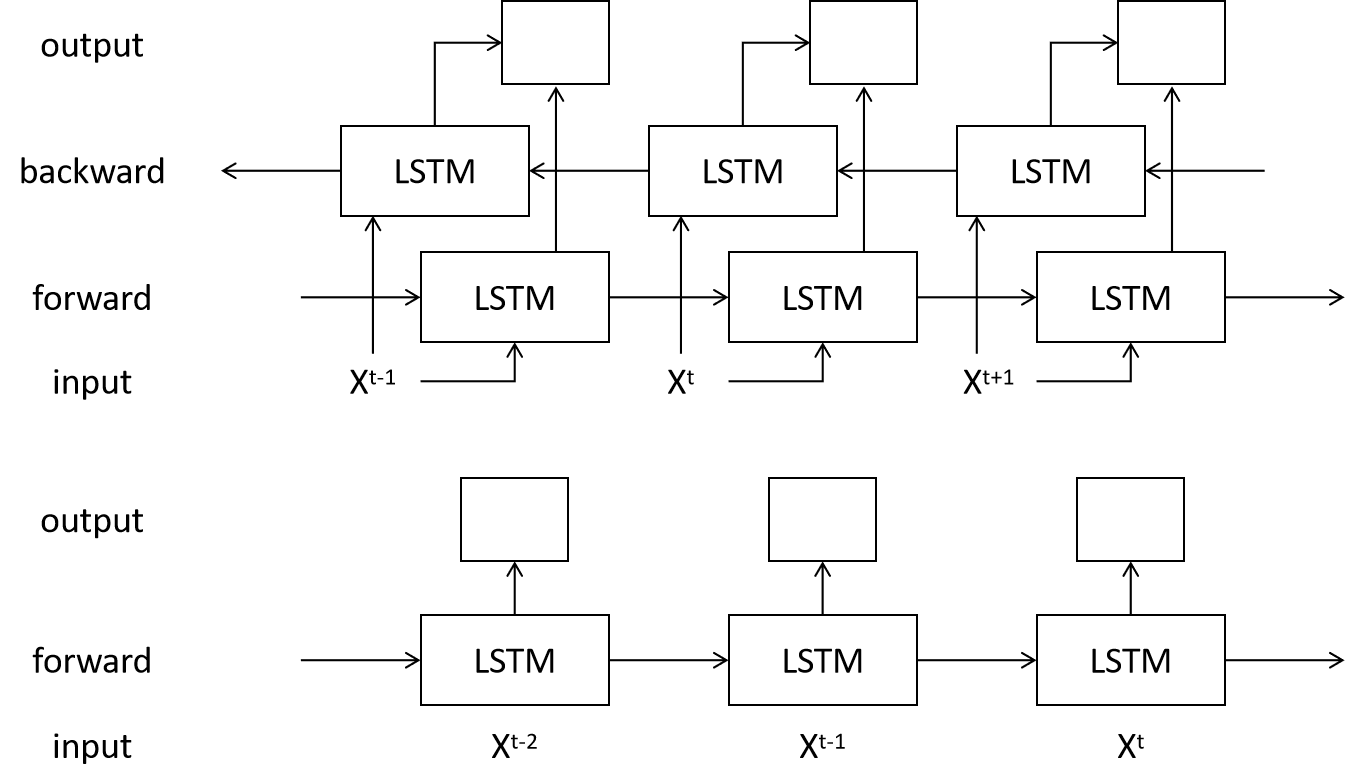
\includegraphics[width=0.9\linewidth]{figures/Fig_lstmcompare.png}
\caption{双向与单向 LSTM 对比示意图。
双向结构(上)在每个时间步同时利用历史与未来帧特征进行建模;
单向结构(下)仅基于历史帧进行递推,以保持因果性并支持流式推理。}
\label{fig_lstmcompare}
\end{figure}

\subsubsection{滑动窗口式自回归训练}

训练时,每段输入为 $N+M$ 帧,前 $N$ 帧作为输入上下文,后 $M$ 帧逐步预测(见图~\ref{fig2_})。
其中,前 $N$ 帧的历史姿态可视为模型的因果历史窗口,
其设计思路与基线模型中附加片段首部的“历史缓冲”类似,
但在意义上有所不同。
CaMN 在双向时间建模下使用该缓冲以补足片段外部上下文,
而 FaceCapGes 则将其重新定义为实时预测所需的前序姿态帧数量,
即当前帧推理所依赖的显式时间上下文。

在训练阶段,模型采用纯自回归(pure autoregressive)方式展开,
即在每一步预测后,将自身生成的历史帧作为下一步输入,
而非采用教师强制(teacher forcing)。
这种方式使模型在优化过程中暴露于自身预测的分布,
保持训练与推理过程的一致性,
避免了教师强制常见的暴露偏差(exposure bias),
即推理阶段模型面对自身生成数据时性能下降的问题。
在每个窗口内连续预测 $M$ 步后,
累计所有预测帧的误差并计算平均损失:
\begin{equation}
\mathcal{L}_{\text{total}} = \frac{1}{M}\sum_{i=1}^{M} \|\hat{\bm{g}}_i - \bm{g}_i\|_2^2.
\end{equation}

虽然该纯自回归方式在训练早期的收敛速度略慢,
但生成稳定性更高,可有效抑制长期序列中的误差积累。
此外,这种机制特别契合实时虚拟人等持续交互场景:
模型在此类应用中并非针对短语段离线生成,
而是与语音流持续同步、长时间运行。
在这种场景下,纯自回归训练使模型在遇到自身预测误差时能够动态修正节奏,
从而在长时间交互中保持自然的动作连续性与节奏稳定性。

每一预测步中定义一个长度为 $N+1$ 的滑动窗口,
其中前 $N$ 帧为输入,第 $N+1$ 帧为预测目标。
形式化定义如下:
\begin{align}
\bm{g}^H_i &= (\bm{g}_{i-N}, ..., \bm{g}_{\min(N, i-1)}) \otimes (\hat{\bm{g}}_{\max(N+1, i-N)}, ..., \hat{\bm{g}}_{i-1}), \\
\hat{\bm{g}}_i &= FaceCapGes(\bm{v}_{i-N}, ..., \bm{v}_i; \bm{g}^H_i),
\end{align}
其中 $\otimes$ 表示时间拼接操作。
该机制在每步仅依赖过去信息,从而保持因果性约束;
同时通过窗口内的滚动更新,在不引入未来帧的前提下实现平滑过渡。
推理阶段模型以单帧为输入流,输出当前时刻的上半身姿态,实现端到端低延迟生成。

需要指出的是,由于滑动窗口机制依赖前 $N$ 帧的上下文信息,
模型在序列开端无法立即生成动作,即存在一个短暂的“冷启动”阶段。
然而在本文的目标应用场景——实时语音驱动虚拟人系统——中,
模型作为常驻进程持续运行,而非针对离散语句反复初始化。
因此该延迟仅在首次启动时出现约 $N$ 帧($0.3$--$0.5$ 秒)的等待,
对用户体验影响可忽略。
这一延迟被视为实时生成框架下的合理权衡。

\begin{figure}[h!t]
\centering
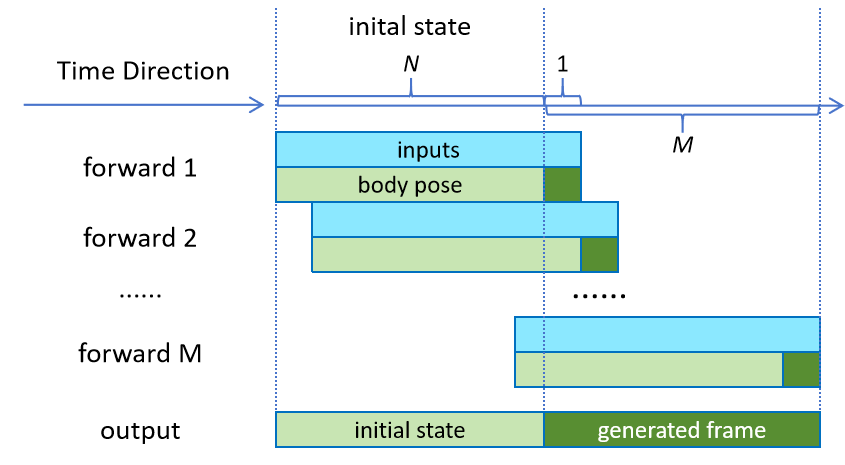
\includegraphics[width=0.75\linewidth]{figures/Fig2.png}
\caption{滑动窗口训练机制:模型通过自回归循环预测 $M$ 帧,每步使用 $N$ 帧上下文并预测第 $N+1$ 帧。损失函数累计所有预测帧的误差,保证因果性与时间平滑性。}
\label{fig2_}
\end{figure}

通过以上适配,FaceCapGes 在保持 CaMN 级联优势的同时显著降低系统延迟,
实现实时稳定的语音与面部驱动手势生成。

然而,仅依赖这两种模态仍存在动作方向与节奏响应不足的问题。
为此,下一节将在级联结构末端引入头部姿态模态,以补充时序反馈与空间方向信号。

\subsection{头部姿态模态的引入与结构位置}
\label{sec:head_encoder}

在模型结构设计中,我们考察了头部姿态特征与其他模态的多种组合方式。%
具体而言,分别尝试了:%
(1) 将头部姿态特征在编码阶段与语音或面部特征进行早期融合;%
(2) 在解码阶段以前两者的嵌入结果为条件,预测头部姿态特征作为辅助信号。%
实验结果显示,这两种交互方式均未带来显著性能提升,%
部分设置甚至出现训练收敛速度下降或动作节奏轻微错位的情况。%

这一现象与认知层面的规律相符。%
头部动作虽然与语音韵律在时间上存在同步性,%
但在认知层面并非由语音或表情直接驱动,%
也难以反向推导这些模态的动态变化。%
换言之,三者更可能属于\emph{并行协同}关系,%
共享节奏与注意机制,但不构成单向的预测链。%

基于此观察,本文在最终架构中采用弱耦合的后级输入设计:%
头部姿态特征在语音与面部特征编码完成后,%
以独立通道的形式拼接至多模态隐向量 $\bm{z}^M_t$,%
而非在编码阶段进行显式交互。%
该处理方式在保持整体结构简洁性的同时,%
仍保留头部姿态在方向、节奏及注意焦点方面的补充作用。%

实验表明,%
在此配置下模型的整体自然度与时序稳定性得到改善,%
说明头部姿态虽非语音或表情的从属模态,%
但作为\emph{空间与节奏的辅助信号}仍具有积极贡献。

\paragraph{输入特征与表示}
本文仅使用头部旋转信息,不引入平移位移特征。BEAT 数据集中演讲者多为站姿,录制中存在身体移动,若直接使用位移作为输入,噪声易混入;此外,目标应用场景中的坐姿用户分布不同,直接建模位移会削弱泛化性。  
因此仅采用旋转特征,并使用连续且可微的 Rot6d 表示,以避免欧拉角与四元数的奇异性问题。

\paragraph{编码器结构}
图~\ref{fig_headencoder} 所示为头部姿态编码器结构。该编码器由两层前馈网络组成,输入为 Rot6d 表示的 6 维向量:
\begin{equation}
\mathbf{z}^{H}_t = E_H(\mathbf{H}_{t-N:t}; \mathbf{z}^A_t, \mathbf{z}^F_t),
\end{equation}
其中 $E_H$ 的具体形式为:
\begin{align}
\mathbf{h}_1 &= \mathrm{ReLU}(W_1 \mathbf{H}_t + b_1), \\
\mathbf{z}^{H}_t &= W_2 \mathbf{h}_1 + b_2,
\end{align}
网络维度设置为:输入 $6$,中间层 $36$,输出 $12$。  
在特征层面,其输出与语音、面部嵌入拼接后输入解码器,形成从语义到反应的多层信号流。

\begin{figure}[h!t]
\centering
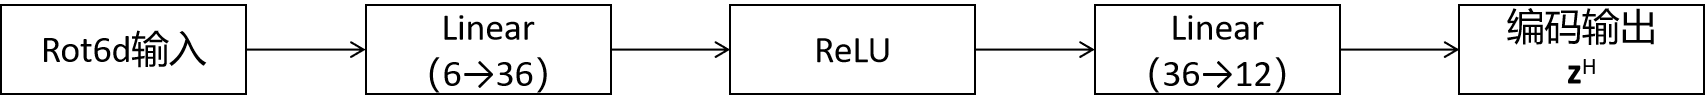
\includegraphics[width=0.8\linewidth]{figures/Fig_headencoder.png}
\caption{头部姿态编码器结构示意图。
输入为 Rot6d 表示的 6 维旋转向量,经两层前馈网络与 ReLU 非线性映射,
输出 12 维紧凑潜在表征。
该编码结果与语音、面部嵌入拼接后输入解码器,用于补充动作的方向与节奏信号。}
\label{fig_headencoder}
\end{figure}

\paragraph{架构位置与实验依据}
在早期实验中,我们尝试将头部姿态与语音、面部特征早期融合,但该方式导致手势方向轻微抖动、语音与动作节奏错位,收敛速度减慢。分析认为,原因在于头部姿态的反应性与非因果性:若过早参与特征交互,会破坏语音—手势因果映射。  
因此本文采用后级融合策略,在语音与面部特征编码完成后再输入头部特征。该设计使模型先形成语义骨架,再由头部姿态进行方向修正与节奏调节。

\subsection{小结:从语义驱动到反应调节的信号层级}

FaceCapGes 在 CaMN 的语音—表情级联架构基础上,通过实时适配与头部模态引入实现了信号层级的扩展。前两级模态承担语义与情感驱动,而新增头部姿态层作为反应性调节模块,在实时条件下为手势提供动态节奏与空间反馈。

\begin{figure*}[h!t]
\centering
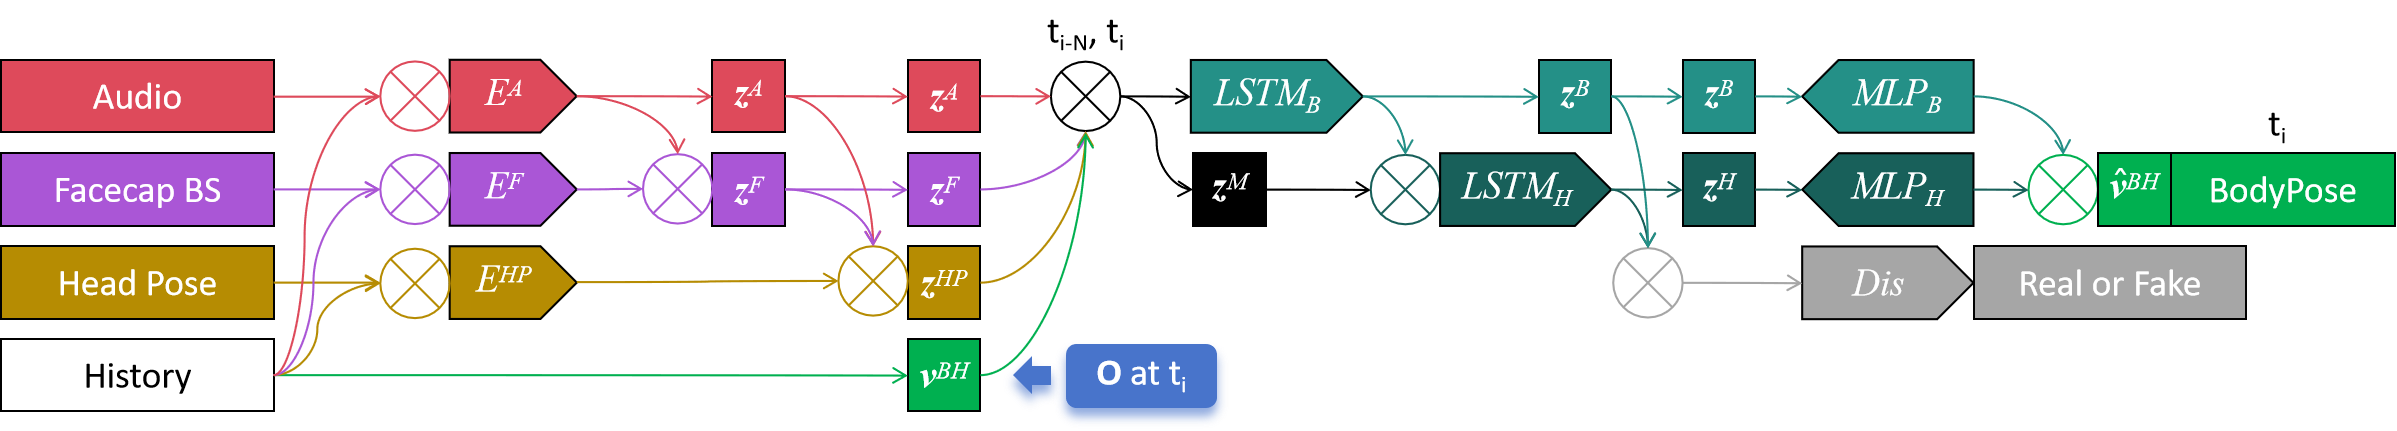
\includegraphics[width=\textwidth]{figures/Fig1.png}
\caption{FaceCapGes 模型结构:音频、面部、头部编码器分别提取模态特征后拼接,输入至 LSTM 解码器生成躯干与手部动作,仅保留最后一帧输出作为当前时刻预测,符合帧级实时推理设定。训练阶段历史姿态序列比目标长度少一帧,需进行零填充。}
\label{fig1_}
\end{figure*}

\section{训练与损失函数设计}
\label{sec:training}

在前述滑动窗口式自回归训练框架下,每段输入序列包含 $N$ 帧上下文与 $M$ 帧预测结果。
模型在每个窗口中输出连续的动作序列 $\hat{\bm{g}} \in \mathbb{R}^{M \times 6 \times 47}$,
并以重构与对抗两类损失共同约束生成质量。

\paragraph{手势重构损失}
重构项 $\mathcal{L}_{Gesture Rec}$ 由位置、速度与加速度误差组成,用以平衡空间准确性与时间平滑性:
\begin{equation}
\bm{g}' = \bm{g}_t - \bm{g}_{t-1}, \quad \bm{g}'' = \bm{g}'_t - \bm{g}'_{t-1},
\end{equation}
\begin{equation}
\mathcal{L}_{Gesture Rec} = \mathcal{L}_{rec}(\bm{g}, \hat{\bm{g}}) + \mathcal{L}_{vel}(\bm{g}', \hat{\bm{g}}') + \mathcal{L}_{acc}(\bm{g}'', \hat{\bm{g}}''),
\end{equation}
其中 $\mathcal{L}_{rec}$ 保证空间姿态重构精度,
$\mathcal{L}_{vel}$ 和 $\mathcal{L}_{acc}$ 强调动态平滑性与时序一致性。
该组合设计在自回归预测中能有效缓解抖动与速度漂移问题。

\paragraph{对抗损失}
为进一步提升动作的自然度,引入对抗项 $\mathcal{L}_{Adv}$:
\begin{equation}
\mathcal{L}_{Adv} = -\mathbb{E}[\log(Dis(\hat{\bm{g}}))],
\end{equation}
其中判别器 $Dis$ 以完整的动作序列为输入,
判别其是否来自真实数据分布。
该项损失约束生成序列的整体动力学分布,
促进生成动作在节奏、加速度和能量变化上与真实表演者一致。
训练中通过交替优化生成器与判别器的参数,保持两者的平衡。

\paragraph{总体损失}
综合两项目标,模型的最终训练目标为:
\begin{equation}
\mathcal{L}_{total} = \mathcal{L}_{Gesture Rec} + \lambda_{adv}\mathcal{L}_{Adv},
\end{equation}
其中 $\lambda_{adv}$ 为对抗损失的权重(实验中设为 $0.1$)。
该设计在保持运动学准确性的同时,提升了时序的自然性与节奏感。

\section{实现与训练配置}
\label{sec:implementation}

在上述训练目标下,FaceCapGes 基于 PyTorch 实现,
所有实验在单张 NVIDIA RTX 4090 GPU 上进行。

本文基于 BEAT 数据集\cite{beatcamn} 进行训练与评估。
该数据集包含多模态同步的语音、面部 blendshape 与全身动作信息,
以 15\,fps 记录多位专业表演者的演讲片段,覆盖多种语义与情绪场景。
其标准骨架结构如图~\ref{fig_beatbones} 所示,
共包含 47 个关节节点。
FaceCapGes 仅预测其中的上半身部分,
包括上肢及躯干的三个主要控制点(蓝色区域所示),
以聚焦语音驱动手势中的表达性动作。
下肢关节保持静态以保证骨架一致性。

\begin{figure}[h!t]
\centering
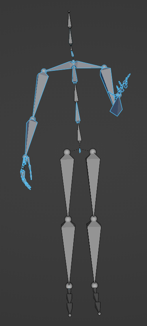
\includegraphics[width=0.15\textwidth]{figures/Fig_BEATBones.png}
\caption{
BEAT 数据集的骨架拓扑结构。
蓝色部分为 FaceCapGes 模型的控制区域,
涵盖上肢与三段脊椎关节,其余节点保持静态。
}
\label{fig_beatbones}
\end{figure}

本文选取表演者 ID~2、4、6、8 的数据进行训练与测试,
其中~2、4~为男性,~6、8~为女性,
确保在性别与说话风格上的分布均衡。
训练集与测试集均包含相同的表演者,
但使用不同的演讲片段,
在预处理阶段已进行严格划分以避免片段交叉。

\paragraph{训练配置}
训练时输入窗口的前序帧数设为 $N=16$,预测长度为 $M=34$,训练片段的切割步长为 10 帧。
相邻片段因此存在部分重叠,从而在保证充分上下文信息的同时提升数据覆盖率与时间连续性。
优化器采用 Adam\cite{adam2017},学习率设为 $2\times10^{-4}$,$\beta_1=0.9, \beta_2=0.999$。
批大小设为 256。
为防止早期训练阶段的不稳定,对抗项在第 10 epoch 后引入,整体训练共 374 个 epoch。
在损失计算中,前 $N$ 帧的历史窗口仅作为因果上下文输入,不参与重构与对抗项的误差回传。
损失函数采用第~\ref{sec:loss} 节所述的复合重构与对抗目标。

\paragraph{姿态表示}
所有身体动作均转换为连续可微的 Rot6d 表示,
使用 EMAGE\cite{emage} 中的实现方法,
以避免欧拉角奇异性与四元数的符号不确定性。

\paragraph{运行性能}
在实时推理阶段,FaceCapGes 能以 15\,FPS 的速度驱动虚拟角色,
满足实时语音交互应用的延迟要求。

\section{本章小结}
本章系统介绍了 FaceCapGes 模型的总体设计与关键技术细节。  
首先,从系统整体出发,阐述了实时语音驱动虚拟人生成管线的总体框架,  
说明了模型在输入采集、手势生成与渲染驱动中的定位与功能。
针对基线模型 CaMN 的结构特征,本文在保持多模态级联优势的基础上,  
对时间建模与实时适配机制进行了系统性改进:  
移除了说话人 ID 输入分支,采用独立模型对应不同说话风格;  
引入单向 LSTM 与滑动窗口式自回归训练以保证因果性与流式生成能力。  

在模型的模态设计上,本文重点分析了语音与面部模态的继承机制,  
并在级联架构末端加入头部姿态编码器,以补充方向性与节奏反馈信号。  
同时,结合对抗优化与多级重构损失,构建了兼顾空间准确性与时间自然性的训练目标。  
实验部分将进一步验证这些结构设计对实时性、平滑性与自然度的提升效果。  
 % !TEX root = ../main.tex

\chapter{评估}

\section{评估设置}

我们使用四种广泛采用的指标对模型进行评估:Fréchet Gesture Distance(FGD)\cite{speech_gesture_generation}、L1 动作多样性(L1DIV)\cite{beatcamn}、节奏对齐度(Beat Alignment, BA)\cite{beatcamn},以及语义相关动作召回率(SRGR)\cite{beatcamn}。所有评估均在 BEAT 数据集上进行,选用说话人编号为 2、4、6 和 8。生成的身体姿态与真实标签均采用相同骨架拓扑的 BVH 格式。FGD 特征由 EMAGE 模型 \cite{emage} 提取,L1DIV、BA 和 SRGR 的实现使用 BEAT 官方提供的代码。所有指标在四位说话人上取平均,以减少个体差异带来的偏差。

\section{客观评估指标与实现细节}
\label{sec:objective_metrics}

为全面评价模型在动作自然性、节奏同步性与多样性等方面的表现,
本文在客观指标层面采用四项度量:Fréchet Gesture Distance (FGD)、Speech–Gesture Rhythm Correlation (SRGR)、Beat Alignment (BA) 以及 L1-based Diversity (L1DIV)。
这些指标分别对应生成动作在分布一致性、语音同步性与变化丰富性等不同维度,
共同构成对模型质量的综合评估体系。

其中,FGD 作为生成分布的核心统计指标,需要训练额外的动作自编码器(AutoEncoder, AE)作为特征提取器;
其余指标则直接基于生成序列与语音信号的时间对应关系进行计算。
本节首先介绍 FGD 的计算原理与评估模型结构,
随后依次阐述其它三项指标的定义与计算方法。

\subsection{Fréchet Gesture Distance (FGD)}
\label{subsec:fgd}

FGD\cite{speech_gesture_generation}用于衡量生成手势分布与真实手势分布之间的统计距离,
灵感源自图像生成领域的 Fréchet Inception Distance (FID)。
不同于图像任务直接利用 Inception 网络特征,
在动作生成领域,特征空间需由单独训练的动作自编码器定义。
该自编码器通过重构任务学习手势的潜在表示,使潜在空间具备对运动模式的压缩与区分能力。
在该潜在空间中,假设真实分布与生成分布的高维嵌入向量分别为
$\mathcal{N}(\bm{\mu}_r, \bm{\Sigma}_r)$ 与 $\mathcal{N}(\bm{\mu}_g, \bm{\Sigma}_g)$,
则 FGD 定义为:
\begin{equation}
\mathrm{FGD} = 
\|\bm{\mu}_r - \bm{\mu}_g\|_2^2 +
\mathrm{Tr}(\bm{\Sigma}_r + \bm{\Sigma}_g - 2(\bm{\Sigma}_r \bm{\Sigma}_g)^{1/2}).
\end{equation}

较小的 FGD 值表示生成动作的统计分布更接近真实数据,
可反映动作的整体自然度与风格一致性。

\paragraph{评估模型结构与训练配置.}
本文在每位说话人的训练集上分别训练一组评估用自编码器,以避免跨说话人分布差异对指标的干扰。
自编码器输入为以 Rot6d 表示的上半身骨架序列,
训练目标为最小化位置、速度与加速度的多尺度重构误差:
\begin{equation}
\mathcal{L}_{AE} = 
\|\hat{\bm{g}} - \bm{g}\|_2^2 +
\lambda_v \|\hat{\bm{g}}' - \bm{g}'\|_2^2 +
\lambda_a \|\hat{\bm{g}}'' - \bm{g}''\|_2^2,
\end{equation}
其中 $\lambda_v = 0.1$, $\lambda_a = 0.1$,$\bm{g}'$、$\bm{g}''$分别为速度与加速度序列。

训练配置如下:
输入片段长度为 32 帧,批大小 256,隐藏层维度 128,学习率 $1.2\times10^{-4}$,优化器为 Adam;
共训练 400 轮。
训练片段步长设为 10,以增加样本数量并保持时间连续性。

\paragraph{骨架拓扑敏感的自编码器.}
在基线模型 CaMN 的 FGD 评估中,使用了基于时间卷积的平铺向量编码器(Embedding-based AutoEncoder)。
该结构将整帧姿态作为高维向量输入,对旋转参数的数值尺度高度敏感,
当使用 Rot6d 表示时,各关节分量的方差差异会在潜在空间中被放大,
导致潜在分布协方差矩阵奇异,从而引起 FGD 数值爆炸。

为避免此问题,本文采用基于骨架拓扑卷积的自编码器(Skeleton-aware AutoEncoder)作为 FGD 特征提取器。
该模型在编码层中引入骨架邻接矩阵 $A$,
通过局部卷积核在相邻关节之间共享权重:
\begin{equation}
\mathbf{h}_i^{(l+1)} = 
\sigma\left(
\sum_{j \in \mathcal{N}(i)} A_{ij} W^{(l)} \mathbf{h}_j^{(l)} + b^{(l)}
\right),
\end{equation}
从而在空间上实现局部归一与结构平滑。
这一设计使特征提取对旋转表示形式不敏感,
可在欧拉角、Axis-Angle 与 Rot6d 等不同表示下保持稳定的潜在分布。
在本文的实验中,该结构显著提高了 FGD 的鲁棒性,
避免了 EmbeddingNet 评估器在 Rot6d 表示下协方差爆炸的现象。

\paragraph{指标计算流程.}
在获得评估模型后,
分别将生成序列与真实序列输入自编码器的编码器部分,
提取潜在特征 $\bm{z}_g$ 与 $\bm{z}_r$,
再计算两者的均值与协方差以求得 FGD。
评估时按说话人独立计算,再取平均值作为总体指标。

\subsection{Speech–Gesture Rhythm Correlation (SRGR)}
\label{subsec:srgr}

SRGR 指标\cite{beatcamn}用于衡量生成手势与语音韵律在节奏层面的同步性,
其核心思想是比较语音能量包络与手势运动速度包络的时间相关程度。
与整句级语义匹配不同,SRGR 反映的是语音与手势在局部时间尺度上的节奏耦合强度。

\paragraph{定义与原理.}
设语音能量序列为 $\bm{e} = \{ e_t \}$,
通过对语音短时能量(Short-Time Energy, STE)进行平滑得到;
手势运动速度定义为各关节旋转向量的一阶差分模长的平均值:
\begin{equation}
v_t = \frac{1}{J}\sum_{j=1}^{J} \|\bm{r}_{t,j} - \bm{r}_{t-1,j}\|_2,
\end{equation}
其中 $J$ 为关节数量,$\bm{r}_{t,j}$ 为第 $j$ 个关节在帧 $t$ 的旋转向量。

对两条时间序列 $\bm{e}$ 与 $\bm{v}$ 进行标准化后,
定义其皮尔逊相关系数(Pearson Correlation)为:
\begin{equation}
\mathrm{SRGR} = \frac{\mathrm{Cov}(\bm{e}, \bm{v})}{\sigma_{\bm{e}}\sigma_{\bm{v}}}.
\end{equation}
SRGR 值越高,表示手势运动节奏与语音节奏的同步程度越强,
通常取值范围在 $[-1, 1]$。
在实际实验中,为减少局部异常的影响,
本文在 1.5 秒滑动窗口内计算局部相关系数并取平均作为最终结果。

\paragraph{计算流程.}
1. 对语音信号计算短时能量,采用窗口长度 50\,ms、步长 10\,ms;  
2. 对生成与真实手势分别计算全身平均运动速度曲线;  
3. 将两条曲线统一至相同时间分辨率并进行归一化;  
4. 滑动计算局部皮尔逊相关系数,最后取平均值作为 SRGR。

该指标能客观反映模型在语音驱动节奏一致性方面的表现,
在主观实验中也与“同步性”评分显著相关。

\subsection{Beat Alignment (BA)}
\label{subsec:ba}

BA(Beat Alignment)指标\cite{beatcamn}用于衡量手势关键动作与语音重读节拍的时间对齐程度,
反映模型在\textbf{时序同步性(temporal synchronization)}方面的性能。
与 SRGR 的全局相关性不同,BA 更注重\textbf{事件级的对齐精度}。

\paragraph{定义与原理.}
设语音节拍集合为 $\mathcal{B}_s = \{t^s_k\}$,
通过检测语音短时能量或梅尔倒谱系数(MFCC)的局部峰值得到;
手势峰集合为 $\mathcal{B}_g = \{t^g_m\}$,
定义为手势速度 $v_t$ 的局部极大点集合。
对于每个语音节拍 $t^s_k$,
计算其最近手势峰的时间差 $\Delta t_k = \min_m |t^s_k - t^g_m|$。
则 BA 指标定义为:
\begin{equation}
\mathrm{BA} = 1 - \frac{1}{K} \sum_{k=1}^{K} \frac{\Delta t_k}{\tau},
\end{equation}
其中 $K$ 为节拍数,$\tau$ 为允许最大偏差阈值(本文取 $\tau=0.5$\,s)。
当 $\Delta t_k < \tau$ 时,记为一次成功对齐。
因此 $\mathrm{BA}$ 越接近 1,表明手势动作越能准确响应语音重读节拍。

\paragraph{计算流程.}
1. 通过能量包络峰值检测获取语音节拍点;  
2. 通过运动速度极值检测获取手势关键帧;  
3. 计算两者的最短时间偏差并归一化;  
4. 平均所有节拍对齐率,得到整体 BA 指标。  

本文使用该指标评估模型在节奏突变与强调语气时的响应能力。
在主观观察中,BA 与视觉上“语音同步自然度”呈正相关。

\subsection{L1-based Diversity (L1DIV)}
\label{subsec:l1div}

L1DIV 指标\cite{beatcamn}衡量生成手势序列的多样性(diversity),
即不同语音输入下模型生成结果的动作差异程度。
该指标反映模型在保持自然性的同时,
能否避免生成收敛到平均动作模式(mode collapse)的倾向。

\paragraph{定义与原理.}
设模型对同一语音片段的 $N$ 次生成结果为
$\{\bm{g}^{(1)}, \bm{g}^{(2)}, \dots, \bm{g}^{(N)}\}$,
则 L1 多样性定义为任意两序列间平均 L1 距离:
\begin{equation}
\mathrm{L1DIV} = 
\frac{2}{N(N-1)} \sum_{i<j} 
\frac{1}{T} \sum_{t=1}^{T} 
\|\bm{g}^{(i)}_t - \bm{g}^{(j)}_t\|_1.
\end{equation}
当 $N=2$ 时,该指标即为两次独立生成的平均动作差异。

\paragraph{计算流程.}
1. 对同一语音输入重复生成多次(不同随机噪声或 dropout 路径);  
2. 对每帧姿态计算关节旋转的 L1 差;  
3. 对时间与样本求平均得到整体 L1DIV 值。  

较高的 L1DIV 表明模型生成具有较强的多样性,
但过高可能意味着动作不稳定或噪声放大。
因此,L1DIV 通常与 FGD 联合分析:  
FGD 反映真实度,L1DIV 反映丰富度,
两者共同平衡模型在自然性—多样性维度上的表现。

\section{模型对比概览}

表~\ref{tab:modalitycomparison} 总结了各模型的输入输出模态特征。值得注意的是,我们的模型是唯一同时支持“头部姿态”输入且完全不依赖未来信息的方案。

\begin{table}[h]
\centering
\resizebox{\linewidth}{!}{%
\begin{tabular}{@{}lccccc|c|c@{}}
\toprule
\multirow{2}{*}{模型} & \multicolumn{5}{c|}{输入模态} & \multirow{2}{*}{未来信息} & \multirow{2}{*}{输出} \\ 
\cmidrule(lr){2-6}
 & 音频 & 面部捕捉 & 头部姿态 & 说话人ID & 情绪 &  &  \\ 
\midrule
CaMN       & $\checkmark$ & $\checkmark$ & $\times$ & $\checkmark$ & $\checkmark$ & $\checkmark$ & 身体 \\
DiffSHEG   & $\checkmark$ & $\times$ & $\times$ & $\checkmark$ & $\times$ & $\checkmark$ & 身体+面部 \\
本方法     & $\checkmark$ & $\checkmark$ & $\checkmark$ & $\ast$ & $\times$ & $\times$ & 身体 \\ 
\bottomrule
\end{tabular}%
}

\section{用户调研}
\label{sec:userstudy}

为进一步验证模型在真实交互环境中的表现,
本文进行了用户主观评估实验,
比较 FaceCapGes、DiffSHEG \cite{diffsheg} 与 CaMN \cite{beatcamn} 三个模型在动作自然性、同步性与多样性方面的主观质量。
本节首先介绍用户研究系统与实验配置,
随后报告主观评价结果与分析。

\subsection{评估系统与实验配置}

\paragraph{实验材料与呈现方式.}
用户评估所使用的手势动画均基于测试集语音片段生成,
并以BVH(Biovision Hierarchy)文件形式保存。
BVH 是一种通用的动作捕捉数据格式,
通过层级化定义骨骼结构与帧级旋转参数,
可直接导入 3D 动画与虚拟人系统。
本文使用的 BVH 文件采用欧拉角旋转表示,以保证与 Unity 的骨骼系统兼容。

由于三种对比模型的输出旋转参数形式不同——
CaMN 模型直接输出欧拉角,
DiffSHEG 输出 Axis-Angle,
而 FaceCapGes 输出 Rot6d 表示——
因此在导出 BVH 之前,
需将后两者统一转换为欧拉角表示,
以便在同一骨架拓扑下进行动画比较。

所有对比模型(FaceCapGes、CaMN、DiffSHEG)均使用相同的训练集与骨骼定义,
其中 CaMN 与 DiffSHEG 采用各自论文公开的原版参数。
虚拟人角色选自 BEAT 数据集提供的公开演讲者模型集合,
并经过 Unity 的 Mecanim 自动骨骼绑定系统匹配。
该系统会自动配对 BVH 文件中定义的骨骼层级与虚拟人模型的骨骼节点,
从而在不依赖手动权重绘制的情况下完成动作重定向。

本系统当前支持的虚拟人模型需同时具备骨骼绑定与 ARKit 兼容的 BlendShape 参数。
基于此约束,实验选用了 CaMN 论文公开的男女两名演讲者模型,二者均满足兼容要求,可实现身体与面部的联合驱动。

\paragraph{播放系统实现.}
我们基于 Unity 自行编写播放脚本,
将各模型生成的 BVH 动画用于驱动虚拟人身体骨骼,
同时以面部捕捉序列驱动 BlendShape 表情参数,
并同步播放原始语音音频。
系统支持同时呈现三种模型生成的动画结果:
用户可在同一画面中(左、中、右)并行观察三种手势表现,
所有语音与面部表情完全一致,
唯一变量为身体动作。
该设计使参与者能够直接比较不同模型在动作风格、
节奏响应与语音同步性方面的差异。

为确保主观评价的公正性与可重复性,
系统在每次实验开始前会随机分配三种模型的位置(左、中、右),
界面上不会显示模型名称,
从而避免潜在偏向。
各测试片段的播放顺序在实验前统一设定,
以保证不同参与者之间的样本顺序均衡。
实验员在播放系统后台记录当前序列与模型对应关系,
以便后续结果统计。

\paragraph{实验界面与设备.}
评估系统提供桌面端与 VR 端两种版本,功能完全一致。
VR 版本基于 PICO 设备实现;
桌面版支持多窗口并行播放,方便用户同时对比。
如图~\ref{fig:userstudy_app} 所示,
播放界面在两种设备上保持统一布局,
播放完成后参与者需通过交互界面对三个模型进行排序打分。
VR 用户在沉浸式环境中逐一观看三段动画;
桌面端用户则可在单屏上同时观察全部模型。
因此前者注重细节感知与临场性,
后者更有利于整体风格与节奏的一致性对比。

\paragraph{实验流程与指导.}
实验正式开始前,
研究人员向参与者说明了三项主观评价标准的含义,
确保所有被试对评分维度理解一致:
\begin{itemize}
    \item \textbf{真实感(Realism)}:整体动作是否自然流畅,是否存在明显的违和感,如朝向异常或突然抖动;
    \item \textbf{同步性(Synchronization)}:手势动作与语调、语音节奏是否协调一致;
    \item \textbf{多样性(Diversity)}:手势是否丰富多变,避免长时间静止或重复单一动作。
\end{itemize}

在实验过程中,
VR 版本于\textbf{线下环境}进行,
桌面版通过\textbf{线上远程环境}执行。
两种形式均保持实时交流通道,
研究人员可在参与者提问时即时解释操作或澄清评分标准。
在正式评估阶段,
参与者可多次重播当前片段,
但不能返回查看先前内容,
以减少记忆偏差。
所有播放条件(\textbf{Unity 场景内的相机角度、光照参数、音量与分辨率设置})
在全部被试中保持一致,
以确保渲染输出的可比性。

需要说明的是,
对于\textbf{VR 实验},
所有测试均在相同的线下实验室环境中进行,
使用同一套 PICO 设备与照明条件;
而\textbf{桌面端实验}通过远程方式执行,
参与者在各自电脑上运行实验程序。
研究人员可通过实时屏幕共享观察其操作流程并保持语音沟通,
但无法严格控制其所在房间的光照或环境噪声条件。
因此,桌面端实验在“观看环境”上存在一定差异,
但由于任务内容与播放系统完全相同,
且实验员在测试中持续指导,
可认为该差异对结果的总体影响有限。

\paragraph{实验材料与任务设计.}
评估样本来自 BEAT 数据集中四位演讲者(ID 2、4、6、8),
其中 2、4 为男性,6、8 为女性。
每位演讲者各选取两段平均长度约 1 分钟的语音片段,
演讲话题互不重复,共组成 \textbf{8 段固定视频样本}。
所有实验均使用相同的 8 段样本,
但其\textbf{呈现顺序在不同被试间经过随机化或平衡化处理},
以避免顺序效应(order effect)。
每段视频均包含三种模型生成的动作版本(FaceCapGes、CaMN、DiffSHEG),
并在播放时随机分配其在屏幕的左右位置。
参与者在观看每个片段后,
根据三项主观标准(真实感、同步性、多样性)
对三个模型的表现进行排序评估。

\begin{figure}[h!t]
\centering
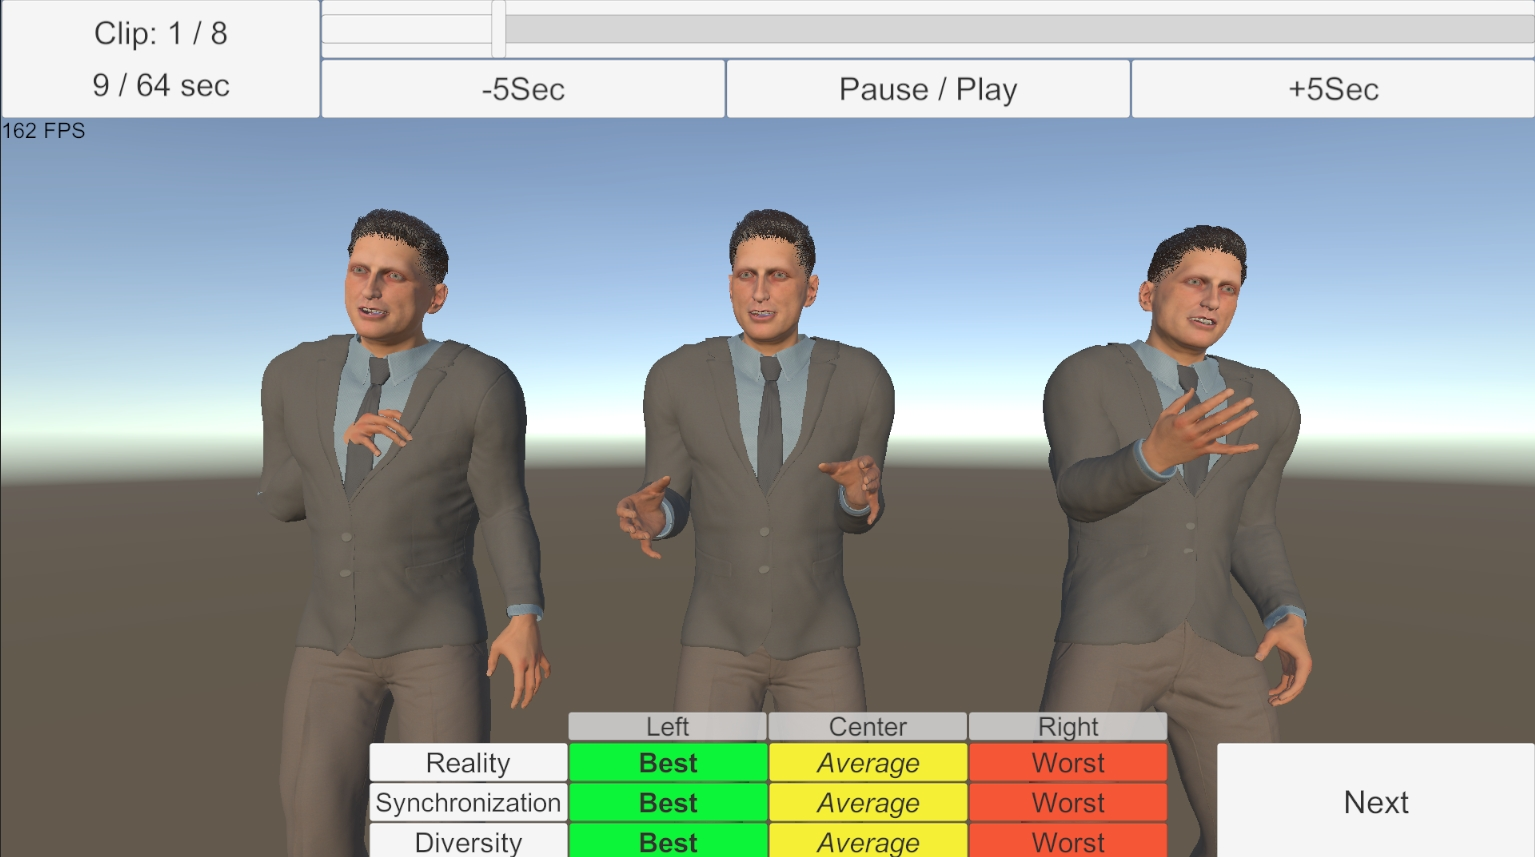
\includegraphics[width=\linewidth]{figures/UserStudyImage.png}
\caption{用户研究系统界面示意图。
左、中、右位置随机分配给三种模型,
音频与面部表情完全一致,仅身体动作不同。}
\label{fig:userstudy_app}
\end{figure}

\paragraph{实验参与者.}
共邀请 16 名参与者(12 名使用 VR 设备,4 名使用桌面端),
涵盖不同性别与学术背景。
所有参与者在实验前均接受了操作说明与校准,
并在系统指导下完成评分练习。
为避免呈现顺序对主观印象造成偏差,
另设计了采用平衡拉丁方(Balanced Latin Square)顺序的实验版本,
使不同参与者观看样本的顺序均衡分布。

\subsection{平衡拉丁方排序设计}
\label{subsec:latin_square}

该版本实验共招募 8 位 VR 用户(4 男 4 女),
排序顺序由 HCI 用户研究工具包 \cite{LatinSquareToolkit} 自动生成,
确保模型与演讲者组合的呈现顺序在全体被试间均匀分布。
所有条件保持一致,唯一变量为视频播放顺序。

\subsection{结果与分析}
\label{subsec:user_study_result}

本节综合分析两轮用户评估的统计结果与参与者反馈。
所有结果均基于相同的 8 段测试样本,
其中模型位置与播放顺序在不同被试间随机化或经平衡拉丁方控制,
以保证主观评价的公正性。

\paragraph{电脑用户测评结果.}
如图~\ref{fig:userstudy} 所示,
在 16 名参与者的总体评价中,
FaceCapGes 在三个维度(真实感、同步性、多样性)上均优于基线模型 CaMN,
并在“真实感”方面与离线扩散模型 DiffSHEG 持平。
这一结果表明,FaceCapGes 虽在严格的实时因果约束下运行,
但仍能保持与非实时生成模型相近的动作自然度与流畅性。

\begin{figure}[h!t]
\centering
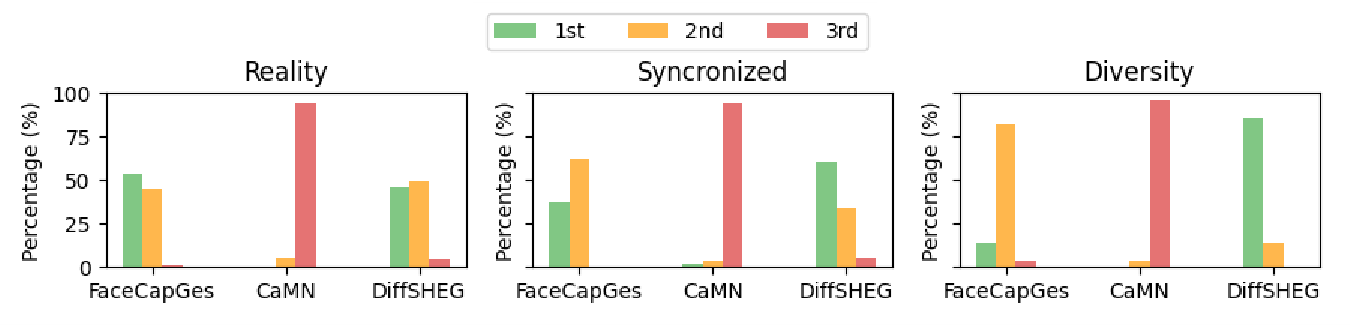
\includegraphics[width=\linewidth]{figures/UserStudy_All.png}
\caption{16 名参与者对三种模型在“真实感”、“同步性”和“多样性”三个维度的主观排名结果。}
\label{fig:userstudy}
\end{figure}

\paragraph{平衡拉丁方实验结果.}
图~\ref{fig:userstudy_latin_square} 展示了平衡拉丁方实验版本中 8 位 VR 用户的独立结果,
该版本严格控制了模型与演讲者组合的呈现顺序。
结果与总体趋势一致,
FaceCapGes 在“同步性”与“真实感”上显著优于 CaMN,
并在“多样性”指标上与 DiffSHEG 接近。
这表明实验结果在不同顺序条件下保持稳定,
进一步验证了模型在多维度主观评价中的一致优势。

\begin{figure}[h!t]
\centering
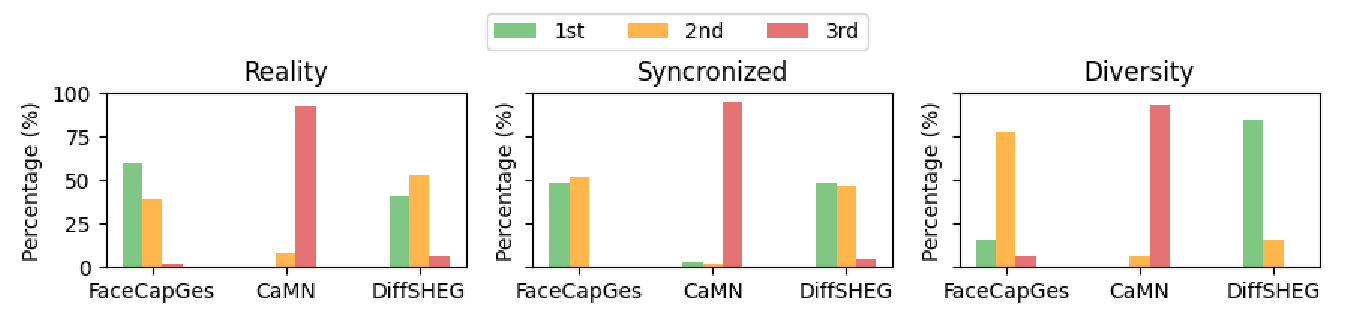
\includegraphics[width=\linewidth]{figures/UserStudy_LatinSquare.png}
\caption{平衡拉丁方实验版本中 8 位 VR 用户的主观排名结果,
评价维度包括“真实感”、“同步性”和“多样性”。}
\label{fig:userstudy_latin_square}
\end{figure}

\paragraph{用户反馈分析.}
根据实验后访谈与自由评论汇总,
参与者普遍认为 FaceCapGes 的动作过渡自然、节奏感强,
手势响应与语音重音、语调变化更加一致。
部分 VR 用户指出,
在沉浸式视角下能够明显感受到手势的连贯性与时序协调,
而 CaMN 在头部与上身动作衔接处偶有“僵硬”或“转向延迟”现象。
约三分之一的参与者提到 DiffSHEG 的动作表现力最强,
但在某些片段中出现手部摆动幅度过大或抖动的情况,
导致同步性评分略低。

桌面端用户普遍认为三种模型的差异在节奏与流畅性上最明显;
VR 用户则更容易察觉动作的空间一致性与临场协调。
两组被试的整体排序趋势一致,
说明模型差异具有跨设备一致性。

\paragraph{结果讨论.}
CaMN 得分较低的主要原因在于其采用欧拉角表示,
导致部分姿态序列在旋转空间中出现不连续,
尤其在头部动作上易产生跳变;
而 DiffSHEG 的高方差输出虽提升了动作多样性,
但表现出一定的突然颤抖,可能来源于Axis-Angle的不连续性。
相比之下,
FaceCapGes 的因果式时间建模和头部姿态融合策略
有效提升了局部动作的平滑性与节奏协调,
使其在实时条件下同时兼顾自然度与稳定性。
此外,
实验的平衡拉丁方版本进一步证明结果在不同呈现顺序下的一致性,
排除了顺序偏差对主观评价的显著影响。

综上,
用户研究表明 FaceCapGes 在实时生成条件下
仍能维持与离线模型相当的主观表现,
在动作真实感、节奏同步性和长时间交互稳定性方面
均显著优于传统因果结构基线,
验证了本文提出的多模态融合与时间建模策略的有效性。

\section{定性分析}

我们强烈建议观看电子附录中的演示视频,内容包含 GT、CaMN、DiffSHEG 与本模型的并排展示,能够直观体现时间对齐性、手势响应性以及头-身协调性方面的差异。

如图~\ref{fig3} 所示,FaceCapGes 能平滑且富有表现力地捕捉说话人动态。与 CaMN 相比,本模型避免了欧拉角带来的不连续问题,生成的身体动作可顺应头部运动趋势。与 DiffSHEG 相比,我们的模型在动作速度上略逊一筹,但能有效避免抖动或夸张姿态。头部姿态的引入也明显提升了手势方向与语义的一致性。

\begin{figure*}[h!t]
\centering
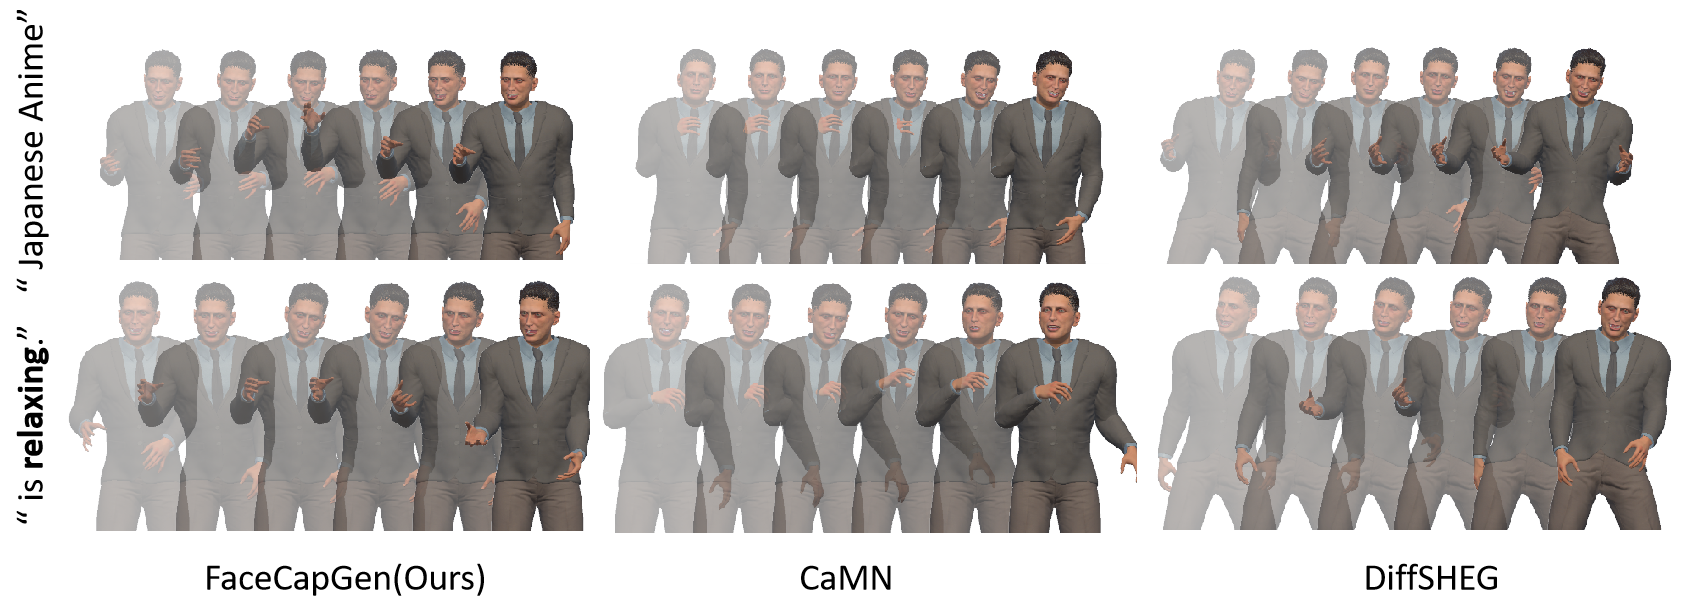
\includegraphics[width=\textwidth]{figures/GeneratedPoseOverview.png}
\caption{GT、CaMN、DiffSHEG 与 FaceCapGes 的动作效果对比。本模型手势响应自然,方向与头部朝向一致。}
\label{fig3}
\end{figure*}

\section{定量分析}

\begin{table*}[h]
\centering
\begin{tabular}{@{}lclrrrr@{}}
\hline
区域 & 方法 & FGD\textdownarrow & SRGR\textuparrow & BA\textuparrow & L1DIV\textuparrow \\
\hline
\multirow{3}{*}{全身}
& CaMN       & 47.732 & 0.098 & 0.845 & 7.591 \\
& DiffSHEG   & \underline{26.846} & \textbf{0.109} & \underline{0.883} & \underline{11.028} \\
& 本方法     & \textbf{23.385} & \underline{0.107} & \textbf{0.913} & \textbf{13.284} \\
\hline
\multirow{3}{*}{不含头部}
& CaMN       & 49.437 & 0.103 & 0.845 & 7.327 \\
& DiffSHEG   & \underline{26.847} & \textbf{0.110} & \underline{0.883} & \underline{10.990} \\
& 本方法     & \textbf{23.384} & \underline{0.107} & \textbf{0.913} & \textbf{13.330} \\
\hline
\end{tabular}
\caption{在 BEAT 四位说话人测试集上的定量评估结果。FaceCapGes 在所有指标上优于 CaMN,且与 DiffSHEG 表现相当。}
\label{tab1}
\end{table*}

表~\ref{tab1} 显示,FaceCapGes 在所有指标上均优于 CaMN。与 DiffSHEG 相比,本模型 FGD 更低,SRGR 相近,且在 L1DIV 上表现最优,表明其生成动作具备良好多样性。但这一结论与用户主观评分存在一定出入:DiffSHEG 在“多样性”上主观排名更高。

这一差异揭示了 L1DIV 的局限性:它主要衡量空间偏离程度,并不能体现动作频率或视觉表现力。虽然我们的模型在结构上更丰富,但用户普遍认为 DiffSHEG 更“活跃”,吸引注意。这说明 L1DIV 无法完全捕捉感知上的丰富性,进一步强调定量与主观评估的互补作用。

\section{消融实验分析}

\begin{table*}[h]
\centering
\begin{tabular}{@{}llrrrr@{}}
\hline
区域 & 变体 & FGD\textdownarrow & SRGR\textuparrow & BA\textuparrow & L1DIV\textuparrow \\
\hline
\multirow{4}{*}{全身}
& CaMN                    & 32.870  & 0.111  & 0.858  & 7.214  \\
& 移除头部姿态           & 19.591  & 0.123  & 0.916  & 10.642 \\
& 移除帧级生成           & 21.592  & \textbf{0.125}  & 0.892  & 10.456 \\
& FaceCapGes(本方法)   & \textbf{19.290}  & 0.123 & \textbf{0.918}  & \textbf{10.871} \\
\hline
\end{tabular}
\caption{说话人 2 的消融实验结果。头部姿态对提升手势自然性与表达力有显著作用。}
\label{tab2}
\end{table*}

表~\ref{tab2} 展示了各模块对模型性能的影响。移除头部姿态会导致所有指标下降,证明其对表达性手势的重要性。

值得注意的是,“非帧级”版本使用未来上下文与双向 LSTM,但其表现反而不及帧级版本。这是因为它采用一次性解码,对每段输入独立处理,无法保证时间连续性,与原 CaMN 的设计一致。而我们的方法通过滑动窗口训练和自回归推理,逐帧依赖历史信息,使动作更连贯、过渡更自然。即使不使用未来帧,也能获得更低的 FGD 和更自然的手势对齐。

\section{性能评估}

\begin{table}[h]
\centering
\begin{tabular}{@{}lr@{}}
\hline
指标 & 时间 \\
\hline
测试帧数 & 93015 (f) \\
推理总时长 & 504 (s) \\
平均单帧时间 & 6.07E-03 (s/f) \\
\hline
\end{tabular}
\caption{在 RTX 4090 上的帧级推理速度评估结果。}
\label{tab3}
\end{table}

为评估实时性能,我们在 BEAT 测试集上使用 batch size 为 1 的配置进行推理测量。如表~\ref{tab3} 所示,模型平均每帧处理时间小于 7 毫秒,满足实时响应需求。

尽管模型推理本身较快,但系统总延迟还受输入特征提取影响。在我们的原型中,音频特征通过 Librosa 离线提取,93,015 帧总计耗时约 61 秒,单帧不足 1 毫秒。实际部署中可替换为如 PyAudio 或 SoundDevice 的实时提取方法,尽管本文未测量其具体延迟。

ARKit 面部追踪的延迟由开发文档估算约为 60FPS \cite{AppleARKitTrackingGuide}。结合模型推理时间,整体系统延迟预计不超过 25ms,足以满足实时虚拟人交互的需求。

 % !TEX root = ../main.tex

\chapter{结论}

本文提出了 FaceCapGes,一种基于 CaMN 框架的帧级实时手势生成模型。与现有离线或依赖未来信息的方法不同,FaceCapGes 可使用户仅通过实时音频、面部 blendshape 权重与头部姿态,即可驱动虚拟角色生成自然手势,无需动作捕捉设备。

本模型融合 LSTM、MLP 以及对抗学习机制,采用级联架构与滑动窗口式自回归训练策略,支持低延迟的在线推理。我们首次将头部姿态作为终端模态引入,有效提升了手势的自然度与协调性。

综合评估表明,FaceCapGes 在生成质量上显著优于 CaMN,并在保持实时性的同时,在主观和客观指标上与主流离线方法表现相当。其模块化设计使其可部署于兼容 ARKit 的轻量设备上,具备良好的实用性与扩展性。

尽管当前系统尚未显式建模语义驱动的手势,未来工作将探索引入语言理解与意图识别机制,以丰富实时交互中的手势语义表达。此外,我们还计划扩展对通用摄像头与非 iOS 平台的支持,通过开发跨平台的面部与姿态捕捉接口,缓解当前对 ARKit 的依赖。

%% !TEX root = ../main.tex

\chapter{数学与引用文献的标注}

\section{数学}

\subsection{数字和单位}

宏包 \pkg{siunitx} 提供了更好的数字和单位支持:
\begin{itemize}
  \item \num{12345.67890}
  \item \complexnum{1+-2i}
  \item \num{.3e45}
  \item \numproduct{1.654 x 2.34 x 3.430}
  \item \unit{kg.m.s^{-1}}
  \item \unit{\micro\meter} $\unit{\micro\meter}$
  \item \unit{\ohm} $\unit{\ohm}$
  \item \numlist{10;20}
  \item \numlist{10;20;30}
  \item \qtylist{0.13;0.67;0.80}{\milli\metre}
  \item \numrange{10}{20}
  \item \qtyrange{10}{20}{\degreeCelsius}
\end{itemize}

\subsection{数学符号和公式}

按照国标 GB/T 3102.11—1993《物理科学和技术中使用的数学符号》,
微分符号 $\dd$ 应使用直立体。除此之外,数学常数也应使用直立体:
\begin{itemize}
  \item 微分符号 $\dd$:\cs{dd}
  \item 圆周率 $\uppi$:\cs{uppi}
  \item 自然对数的底 $\ee$:\cs{ee}
  \item 虚数单位 $\ii$, $\jj$:\cs{ii} \cs{jj}
\end{itemize}

公式应另起一行居中排版。公式后应注明编号,按章顺序编排,编号右端对齐。
\begin{equation}
  \ee^{\ii\uppi} + 1 = 0,
\end{equation}
\begin{equation}
  \frac{\dd^2 u}{\dd t^2} = \int f(x) \dd x.
\end{equation}

公式末尾是需要添加标点符号的,至于用逗号还是句号,取决于公式下面一句是接着公式说的,还是另起一句。
\begin{equation}
  \frac{2h}{\pi}\int_{0}^{\infty}\frac{\sin\left( \omega\delta \right)}{\omega}
  \cos\left( \omega x \right) \dd\omega = 
  \begin{cases}
    h, & \left| x \right| < \delta, \\
    \frac{h}{2}, & x = \pm \delta, \\
    0, & \left| x \right| > \delta.
  \end{cases}
\end{equation}
公式较长时最好在等号“$=$”处转行。
\begin{align}
    & I (X_3; X_4) - I (X_3; X_4 \mid X_1) - I (X_3; X_4 \mid X_2) \nonumber \\
  = & [I (X_3; X_4) - I (X_3; X_4 \mid X_1)] - I (X_3; X_4 \mid \tilde{X}_2) \\
  = & I (X_1; X_3; X_4) - I (X_3; X_4 \mid \tilde{X}_2).
\end{align}

如果在等号处转行难以实现,也可在 $+$、$-$、$\times$、$\div$ 运算符号处转行,转行
时运算符号仅书写于转行式前,不重复书写。
\begin{multline}
  \frac{1}{2} \Delta (f_{ij} f^{ij}) =
    2 \left(\sum_{i<j} \chi_{ij}(\sigma_{i} - \sigma_{j})^{2}
    + f^{ij} \nabla_{j} \nabla_{i} (\Delta f) \right. \\
  \left. + \nabla_{k} f_{ij} \nabla^{k} f^{ij} +
    f^{ij} f^{k} \left[2\nabla_{i}R_{jk}
    - \nabla_{k} R_{ij} \right] \vphantom{\sum_{i<j}} \right).
\end{multline}

\subsection{定理环境}

示例文件中使用 \pkg{ntheorem} 宏包配置了定理、引理和证明等环境。用户也可以使用
\pkg{amsthm} 宏包。

这里举一个“定理”和“证明”的例子。
\begin{theorem}[留数定理]
\label{thm:res}
  假设 $U$ 是复平面上的一个单连通开子集,$a_1, \ldots, a_n$ 是复平面上有限个点,
  $f$ 是定义在 $U \backslash \{a_1, \ldots, a_n\}$ 上的全纯函数,如果 $\gamma$
  是一条把 $a_1, \ldots, a_n$ 包围起来的可求长曲线,但不经过任何一个 $a_k$,并且
  其起点与终点重合,那么:

  \begin{equation}
    \label{eq:res}
    \oint\limits_\gamma f(z)\, \dd z = 2\uppi \ii \sum_{k=1}^n \operatorname{I}(\gamma, a_k) \operatorname{Res}(f, a_k).
  \end{equation}

  如果 $\gamma$ 是若尔当曲线,那么 $\operatorname{I}(\gamma, a_k) = 1$,因此:

  \begin{equation}
    \label{eq:resthm}
    \oint\limits_\gamma f(z)\, \dd z = 2\uppi \ii \sum_{k=1}^n \operatorname{Res}(f, a_k).
  \end{equation}

  在这里,$\operatorname{Res}(f, a_k)$ 表示 $f$ 在点 $a_k$ 的留数,
  $\operatorname{I}(\gamma, a_k)$ 表示 $\gamma$ 关于点 $a_k$ 的卷绕数。卷绕数是
  一个整数,它描述了曲线 $\gamma$ 绕过点 $a_k$ 的次数。如果 $\gamma$ 依逆时针方
  向绕着 $a_k$ 移动,卷绕数就是一个正数,如果 $\gamma$ 根本不绕过 $a_k$,卷绕数
  就是零。

  定理~\ref{thm:res} 的证明。

  \begin{proof}
    首先,由……

    其次,……

    所以……
  \end{proof}
\end{theorem}

\section{引用文献的标注}

按照教务处的要求,参考文献外观应符合国标 GB/T 7714 的要求。模版使用 \BibLaTeX{}
配合 \pkg{biblatex-gb7714-2015} 样式包%
\footnote{\url{https://www.ctan.org/pkg/biblatex-gb7714-2015}}%
控制参考文献的输出样式,后端采用 \pkg{biber} 管理文献。

请注意 \pkg{biblatex-gb7714-2015} 宏包 2016 年 9 月才加入 CTAN,如果你使用的
\TeX{} 系统版本较旧,可能没有包含 \pkg{biblatex-gb7714-2015} 宏包,需要手动安装。
\BibLaTeX{} 与 \pkg{biblatex-gb7714-2015} 目前在活跃地更新,为避免一些兼容性问
题,推荐使用较新的版本。

正文中引用参考文献时,使用 \verb|\cite{key1,key2,key3...}| 可以产生“上标引用的参
考文献”,如 \cite{Yu2001,Cheng1999,LSC1957}。使用
\verb|\parencite{key1,key2,key3...}| 则可以产生水平引用的参考文献,例如
\parencite{Li1999,Jiang1989,Hopkinson1999}。请看下面的例子,将会穿插使用水平的和
上标的参考文献:普通图书\parencite{Yu2001,Jiang1998},论文集、会议录
\cite{CSTAM1990},科技报告\parencite{WHO1970},学位论文\cite{Zhang1998},专利文
献\parencite{Jiang1989,HBLZ2001},专著中析出的文献\cite{Cheng1999,GBT2659},期刊
中析出的文献\parencite{Li1999,Li2000},报纸中析出的文献\cite{Ding2000}, 电子文献
\parencite{Jiang1999,Christine1998,Xiao2001}。

可以使用 \verb|\nocite{key1,key2,key3...}| 将参考文献条目加入到文献表中但不在正
文中引用。使用 \verb|\nocite{*}| 可以将参考文献数据库中的所有条目加入到文献表
中。
\nocite{Yang1999,Schinstock2000,Wen1990,GBT16159}

%% !TeX root = ../main.tex

\chapter{浮动体}

\section{插图}

插图功能是利用 \TeX{} 的特定编译程序提供的机制实现的,不同的编译程序支持不同的图
形方式。有的同学可能听说“\LaTeX{} 只支持 EPS”,事实上这种说法是不准确的。\XeTeX{}
可以很方便地插入 EPS、PDF、PNG、JPEG 格式的图片。

一般图形都是处在浮动环境中。之所以称为浮动是指最终排版效果图形的位置不一定与源文
件中的位置对应,这也是刚使用 \LaTeX{} 同学可能遇到的问题。如果要强制固定浮动图形
的位置,请使用 \pkg{float} 宏包,它提供了 \texttt{[H]} 参数。

\subsection{单个图形}

图要有图题,研究生图题采用中英文对照,并置于图的编号之后,图的编号和图题应置于图
下方的居中位置。引用图应在图题右上角标出文献来源。当插图中组成部件由数字或字母等
编号表示时,可在插图下方添加图注进行说明,如图~\ref{fig:cn_100t} 所示。

\begin{figure}[!htp]
  \centering
  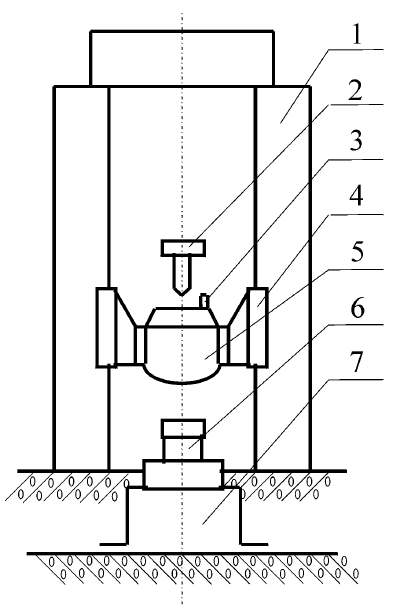
\includegraphics[width=4cm]{cn_100t.png} \\
    1.立柱 2.提升释放机构 3.标准冲击加速度计 \\
    4.导轨 5.重锤 6.被校力传感器 7.底座 \\
  \bicaption[出现在插图索引中]
    {单个图形示例\cite{He1999}。如果表格的标题很长,那么在表格索引中就会很不美观。可
      以在前面用中括号写一个简短的标题,这个标题会出现在索引中。}
    {Stay hungry, stay foolish.}
  \label{fig:cn_100t}
\end{figure}

\subsection{多个图形}

简单插入多个图形的例子如图~\ref{fig:SRR} 所示。这两个水平并列放置的子图共用一个
图形计数器,没有各自的子图题。


\begin{figure}[!htp]
  \centering
  
\includegraphics[height=2cm]{sjtu-vi-badge-blue.pdf}
  \hspace{1cm}
  
\includegraphics[height=2cm]{sjtu-vi-badge-blue.pdf}
  \bicaption{中文题图}{English caption}
  \label{fig:SRR}
\end{figure}

如果多个图形相互独立,并不共用一个图形计数器,那么用 \texttt{minipage} 或者
\texttt{parbox} 就可以,如图~\ref{fig:parallel1} 与图~\ref{fig:parallel2}。

\begin{figure}[!htp]
  \centering
  \begin{minipage}{0.48\textwidth}
    \centering
    
\includegraphics[height=1.5cm]{sjtu-vi-name-blue.pdf}
    \caption{并排第一个图}
    \label{fig:parallel1}
  \end{minipage}\hfill
  \begin{minipage}{0.48\textwidth}
    \centering
    
\includegraphics[height=1.5cm]{sjtu-vi-name-blue.pdf}
    \caption{并排第二个图}
    \label{fig:parallel2}
  \end{minipage}
\end{figure}

如果要为共用一个计数器的多个子图添加子图题,建议使用较新的 \pkg{subcaption}宏
包,不建议使用 \pkg{subfigure} 或 \pkg{subfig} 等宏包。

推荐使用 \pkg{subcaption} 宏包的 \cs{subcaptionbox} 并排子图,子图题置于子图之
下,子图号用 a)、b) 等表示。也可以使用 \pkg{subcaption} 宏包的 \cs{subcaption}
(放在 minipage中,用法同 \cs{caption})。

\pkg{subcaption} 宏包也提供了 \pkg{subfigure} 和 \pkg{subtable} 环境,如
图~\ref{fig:subfigure}。

\begin{figure}[!htp]
  \centering
  \begin{subfigure}{0.3\textwidth}
    \centering
    
\includegraphics[height=2cm]{sjtu-vi-badge-blue.pdf}
    \caption{校徽}
  \end{subfigure}
  \hspace{1cm}
  \begin{subfigure}{0.4\textwidth}
    \centering
    
\includegraphics[height=1.5cm]{sjtu-vi-name-blue.pdf}
    \caption{校名。注意这个图略矮些,subfigure 中同一行的子图在顶端对齐。}
  \end{subfigure}
  \caption{包含子图题的范例(使用 subfigure)}
  \label{fig:subfigure}
\end{figure}

搭配 \pkg{bicaption} 宏包时,可以启用 \cs{subcaptionbox} 和 \cs{subcaption} 的双
语变种 \cs{bisubcaptionbox} 和 \cs{bisubcaption},如图~\ref{fig:bisubcaptionbox}
所示。

\begin{figure}[!hbtp]
  \centering
  \bisubcaptionbox{$R_3 = 1.5\text{mm}$ 时轴承的压力分布云图}%
                  {Pressure contour of bearing when $R_3 = 1.5\text{mm}$}%
                  [6.4cm]{\includegraphics[height=3cm]{example-image-a.pdf}}
  \hspace{1cm}
  \bisubcaptionbox{$R_3 = 2.5\text{mm}$ 时轴承的压力分布云图}%
                  {Pressure contour of bearing when $R_3 = 2.5\text{mm}$}%
                  [6.4cm]{\includegraphics[height=3cm]{example-image-b.pdf}}
  \bicaption{包含子图题的范例(使用 subcaptionbox)}
            {Example with subcaptionbox}
  \label{fig:bisubcaptionbox}
\end{figure}


\section{表格}

\subsection{基本表格}

编排表格应简单明了,表达一致,明晰易懂,表文呼应、内容一致。表题置于表上,研究生
学位论文可以用中、英文两种文字居中排写,中文在上,也可以只用中文。

表格的编排建议采用国际通行的三线表\footnote{三线表,以其形式简洁、功能分明、阅读
方便而在科技论文中被推荐使用。三线表通常只有 3 条线,即顶线、底线和栏目线,没有
竖线。}。三线表可以使用 \pkg{booktabs} 提供的 \cs{toprule}、\cs{midrule} 和
\cs{bottomrule}。它们与 \pkg{longtable} 能很好的配合使用。

\begin{table}[!hpt]
  \caption[一个颇为标准的三线表]{一个颇为标准的三线表\footnotemark}
  \label{tab:firstone}
  \centering
  \begin{tabular}{@{}llr@{}} \toprule
    \multicolumn{2}{c}{Item} \\ \cmidrule(r){1-2}
    Animal & Description & Price (\$)\\ \midrule
    Gnat  & per gram  & 13.65 \\
          & each      & 0.01 \\
    Gnu   & stuffed   & 92.50 \\
    Emu   & stuffed   & 33.33 \\
    Armadillo & frozen & 8.99 \\ \bottomrule
  \end{tabular}
\end{table}
\footnotetext{这个例子来自
  \href{https://mirrors.sjtug.sjtu.edu.cn/ctan/macros/latex/contrib/booktabs/booktabs.pdf}%
  {《Publication quality tables in LaTeX》}(\pkg{booktabs} 宏包的文档)。这也是
  一个在表格中使用脚注的例子,请留意与 \pkg{threeparttable} 实现的效果有何不
  同。}

\subsection{复杂表格}

我们经常会在表格下方标注数据来源,或者对表格里面的条目进行解释。可以用
\pkg{threeparttable} 实现带有脚注的表格,如表~\ref{tab:footnote}。

\begin{table}[!htpb]
  \bicaption{一个带有脚注的表格的例子}{A Table with footnotes}
  \label{tab:footnote}
  \centering
  \begin{threeparttable}[b]
     \begin{tabular}{ccd{4}cccc}
      \toprule
      \multirow{2}*{total} & \multicolumn{2}{c}{20\tnote{a}} & \multicolumn{2}{c}{40} & \multicolumn{2}{c}{60} \\
      \cmidrule(lr){2-3}\cmidrule(lr){4-5}\cmidrule(lr){6-7}
      & www & \multicolumn{1}{c}{k} & www & k & www & k \\ % 使用说明符 d 的列会自动进入数学模式,使用 \multicolumn 对文字表头做特殊处理
      \midrule
      & $\underset{(2.12)}{4.22}$ & 120.0140\tnote{b} & 333.15 & 0.0411 & 444.99 & 0.1387 \\
      & 168.6123 & 10.86 & 255.37 & 0.0353 & 376.14 & 0.1058 \\
      & 6.761    & 0.007 & 235.37 & 0.0267 & 348.66 & 0.1010 \\
      \bottomrule
    \end{tabular}
    \begin{tablenotes}
    \item [a] the first note.
    \item [b] the second note.
    \end{tablenotes}
  \end{threeparttable}
\end{table}

如某个表需要转页接排,可以用 \pkg{longtable} 实现。接排时表题省略,表头应重复书
写,并在右上方写“续表 xx”,如表~\ref{tab:performance}。

\begin{ThreePartTable}
  \begin{TableNotes}
    \item[a] 一个脚注
    \item[b] 另一个脚注
  \end{TableNotes}
  \begin{longtable}[c]{c*{6}{r}}
    \bicaption{实验数据}{Experimental data}
    \label{tab:performance} \\
    \toprule
    测试程序 & \multicolumn{1}{c}{正常运行} & \multicolumn{1}{c}{同步}
      & \multicolumn{1}{c}{检查点} & \multicolumn{1}{c}{卷回恢复}
      & \multicolumn{1}{c}{进程迁移} & \multicolumn{1}{c}{检查点} \\
    & \multicolumn{1}{c}{时间 (s)} & \multicolumn{1}{c}{时间 (s)}
      & \multicolumn{1}{c}{时间 (s)} & \multicolumn{1}{c}{时间 (s)}
      & \multicolumn{1}{c}{时间 (s)} &  文件(KB)\\
    \midrule
    \endfirsthead
    \multicolumn{7}{l}{\textbf{续表~\thetable}} \\
    % 英语论文:\multicolumn{7}{r}{\textbf{Table~\thetable~(continued)}} \\
    \toprule
    测试程序 & \multicolumn{1}{c}{正常运行} & \multicolumn{1}{c}{同步}
      & \multicolumn{1}{c}{检查点} & \multicolumn{1}{c}{卷回恢复}
      & \multicolumn{1}{c}{进程迁移} & \multicolumn{1}{c}{检查点} \\
    & \multicolumn{1}{c}{时间 (s)} & \multicolumn{1}{c}{时间 (s)}
      & \multicolumn{1}{c}{时间 (s)} & \multicolumn{1}{c}{时间 (s)}
      & \multicolumn{1}{c}{时间 (s)}&  文件(KB)\\
    \midrule
    \endhead
    \hline
    \multicolumn{7}{r}{续下页}
    \endfoot
    \insertTableNotes
    \endlastfoot
    CG.A.2 & 23.05 & 0.002 & 0.116 & 0.035 & 0.589 & 32491 \\
    CG.A.4 & 15.06 & 0.003 & 0.067 & 0.021 & 0.351 & 18211 \\
    CG.A.8 & 13.38 & 0.004 & 0.072 & 0.023 & 0.210 & 9890 \\
    CG.B.2 & 867.45 & 0.002 & 0.864 & 0.232 & 3.256 & 228562 \\
    CG.B.4 & 501.61 & 0.003 & 0.438 & 0.136 & 2.075 & 123862 \\
    CG.B.8 & 384.65 & 0.004 & 0.457 & 0.108 & 1.235 & 63777 \\
    MG.A.2 & 112.27 & 0.002 & 0.846 & 0.237 & 3.930 & 236473 \\
    MG.A.4 & 59.84 & 0.003 & 0.442 & 0.128 & 2.070 & 123875 \\
    MG.A.8 & 31.38 & 0.003 & 0.476 & 0.114 & 1.041 & 60627 \\
    MG.B.2 & 526.28 & 0.002 & 0.821 & 0.238 & 4.176 & 236635 \\
    MG.B.4 & 280.11 & 0.003 & 0.432 & 0.130 & 1.706 & 123793 \\
    MG.B.8 & 148.29 & 0.003 & 0.442 & 0.116 & 0.893 & 60600 \\
    LU.A.2 & 2116.54 & 0.002 & 0.110 & 0.030 & 0.532 & 28754 \\
    LU.A.4 & 1102.50 & 0.002 & 0.069 & 0.017 & 0.255 & 14915 \\
    LU.A.8 & 574.47 & 0.003 & 0.067 & 0.016 & 0.192 & 8655 \\
    LU.B.2 & 9712.87 & 0.002 & 0.357 & 0.104 & 1.734 & 101975 \\
    LU.B.4 & 4757.80 & 0.003 & 0.190 & 0.056 & 0.808 & 53522 \\
    LU.B.8 & 2444.05 & 0.004 & 0.222 & 0.057 & 0.548 & 30134 \\
    EP.A.2 & 123.81 & 0.002 & 0.010 & 0.003 & 0.074 & 1834 \\
    EP.A.4 & 61.92 & 0.003 & 0.011 & 0.004 & 0.073 & 1743 \\
    EP.A.8 & 31.06 & 0.004 & 0.017 & 0.005 & 0.073 & 1661 \\
    EP.B.2 & 495.49 & 0.001 & 0.009 & 0.003 & 0.196 & 2011 \\
    EP.B.4 & 247.69 & 0.002 & 0.012 & 0.004 & 0.122 & 1663 \\
    EP.B.8 & 126.74 & 0.003 & 0.017 & 0.005 & 0.083 & 1656 \\
    SP.A.2 & 123.81 & 0.002 & 0.010 & 0.003 & 0.074 & 1854 \\
    SP.A.4 & 51.92 & 0.003 & 0.011 & 0.004 & 0.073 & 1543 \\
    SP.A.8 & 31.06 & 0.004 & 0.017 & 0.005 & 0.073 & 1671 \\
    SP.B.2 & 495.49 & 0.001 & 0.009 & 0.003 & 0.196 & 2411 \\
    SP.B.4 \tnote{a} & 247.69 & 0.002 & 0.014 & 0.006 & 0.152 & 2653 \\
    SP.B.8 \tnote{b} & 126.74 & 0.003 & 0.017 & 0.005 & 0.082 & 1755 \\
    \bottomrule
  \end{longtable}
\end{ThreePartTable}

\section{算法环境}

算法环境可以使用 \pkg{algorithms} 宏包或者较新的 \pkg{algorithm2e} 实现。
算法~\ref{algo:algorithm} 是一个使用 \pkg{algorithm2e} 的例子。关于排版算法环境
的具体方法,请阅读相关宏包的官方文档。

\begin{algorithm}[htb]
  \caption{算法示例}
  \label{algo:algorithm}
  \small
  \SetAlgoLined
  \KwData{this text}
  \KwResult{how to write algorithm with \LaTeXe }

  initialization\;
  \While{not at end of this document}{
    read current\;
    \eIf{understand}{
      go to next section\;
      current section becomes this one\;
    }{
      go back to the beginning of current section\;
    }
  }
\end{algorithm}

\section{代码环境}

我们可以在论文中插入算法,但是不建议插入大段的代码。如果确实需要插入代码,建议使
用 \pkg{listings} 宏包。

\begin{codeblock}[language=C]
#include <stdio.h>
#include <unistd.h>
#include <sys/types.h>
#include <sys/wait.h>

int main() {
  pid_t pid;

  switch ((pid = fork())) {
  case -1:
    printf("fork failed\n");
    break;
  case 0:
    /* child calls exec */
    execl("/bin/ls", "ls", "-l", (char*)0);
    printf("execl failed\n");
    break;
  default:
    /* parent uses wait to suspend execution until child finishes */
    wait((int*)0);
    printf("is completed\n");
    break;
  }

  return 0;
}
\end{codeblock}

%% !TEX root = ../main.tex

\chapter{全文总结}

这里是全文总结内容。

2015 年 2 月 28 日,中央在北京召开全国精神文明建设工作表彰暨学雷锋志愿服务大会,
公布全国文明城市(区)、文明村镇、文明单位名单。上海交通大学荣获全国文明单位称
号。

全国文明单位这一荣誉是对交大人始终高度重视文明文化工作的肯定,是对交大长期以来文
明创建工作成绩的褒奖。在学校党委、文明委的领导下,交大坚持将文明创建工作纳入学校
建设世界一流大学的工作中,全体师生医护员工群策群力、积极开拓,落实国家和上海市有
关文明创建的各项要求,以改革创新、科学发展为主线,以质量提升为目标,聚焦文明创建
工作出现的重点和难点,优化文明创建工作机制,传播学校良好形象,提升社会美誉度,显
著增强学校软实力。2007 至 2012 年间,上海交大连续三届荣获“上海市文明单位”称
号,成为创建全国文明单位的新起点。

上海交大自启动争创全国文明单位工作以来,凝魂聚气、改革创新,积极培育和践行社会主
义核心价值观。坚持统筹兼顾、多措并举,将争创全国文明单位与学校各项中心工作紧密结
合,着力构建学校文明创建新格局,不断提升师生医护员工文明素养,以“冲击世界一流大
学汇聚强大精神动力”为指导思想,以“聚焦改革、多元推进、以评促建、丰富内涵、彰显
特色”为工作原则,并由全体校领导群策领衔“党的建设深化、思想教育深入、办学成绩显
著、大学文化丰富、校园环境优化、社会责任担当”六大板块共 28 项重点突破工作,全面
展现近年来交大文明创建工作的全貌和成就。

进入新阶段,学校将继续开拓文明创建工作新格局,不断深化工作理念和工作实践,创新工
作载体、丰富活动内涵、凸显创建成效,积极服务于学校各项中心工作和改革发展的大局
面,在上级党委、文明委的关心下,在学校党委的直接领导下,与时俱进、开拓创新,为深
化内涵建设、加快建成世界一流大学、推动国家进步和社会发展而努力奋斗!

上海交通大学医学院附属仁济医院也获得全国文明单位称号。


%TC:ignore

% 参考文献
\printbibliography[heading=bibintoc]

% 附录
\appendix

% 附录中图表不加入索引
\captionsetup{list=no}

% 附录内容
% !TEX root = ../main.tex

\chapter{平衡拉丁方排序设计}

为进一步控制呈现顺序带来的偏差,我们设计并实施了用户研究的另一版本,采用 HCI 用户研究工具包 \cite{LatinSquareToolkit} 生成的平衡拉丁方(Balanced Latin Square)排序。本实验版本共招募 8 位参与者(4 名男性,4 名女性),全部使用 VR 头显设备,以构建性别平衡的样本组。如图~\ref{fig:userstudy_latin_square} 所示,展示了该版本用户在“真实感”、“同步性”和“多样性”三个维度上的评分结果。

\begin{figure}[h]
\centering
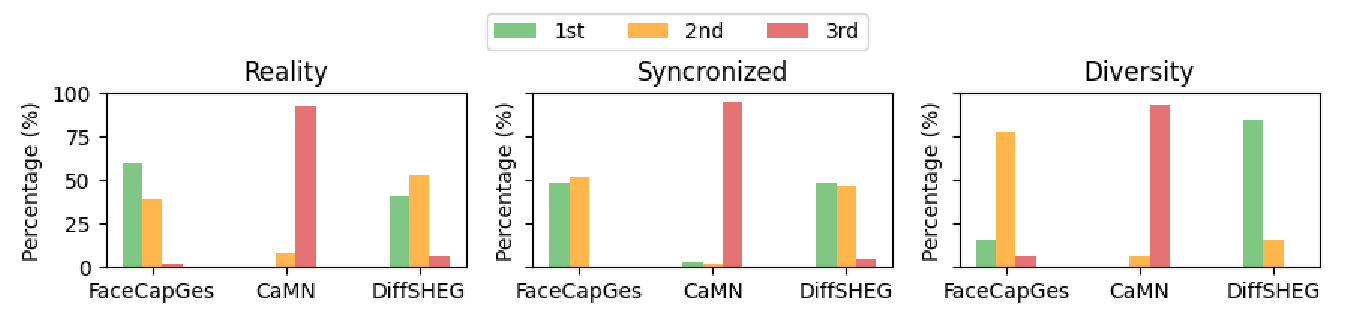
\includegraphics[width=\linewidth]{figures/UserStudy_LatinSquare.png}
\caption{平衡拉丁方实验版本中的用户主观评分结果,共 8 位参与者,评价维度包括“真实感”、“同步性”和“多样性”。}
\label{fig:userstudy_latin_square}
\end{figure}

本研究中所用播放界面如图~\ref{fig:userstudy_app} 所示。该界面在 VR 与桌面端中保持一致,使参与者能够以随机顺序观看三种模型(FaceCapGes(本方法)、DiffSHEG \cite{diffsheg}、CaMN \cite{beatcamn})生成的手势动画。用户可多次重播当前片段,但不能返回浏览先前内容。在每段视频播放结束后,参与者通过拖动界面下方的评分面板,对三个模型进行排序打分。该界面同样适用于平衡拉丁方实验版本,确保所有参与者使用统一的评估流程。

\begin{figure}[h]
\centering
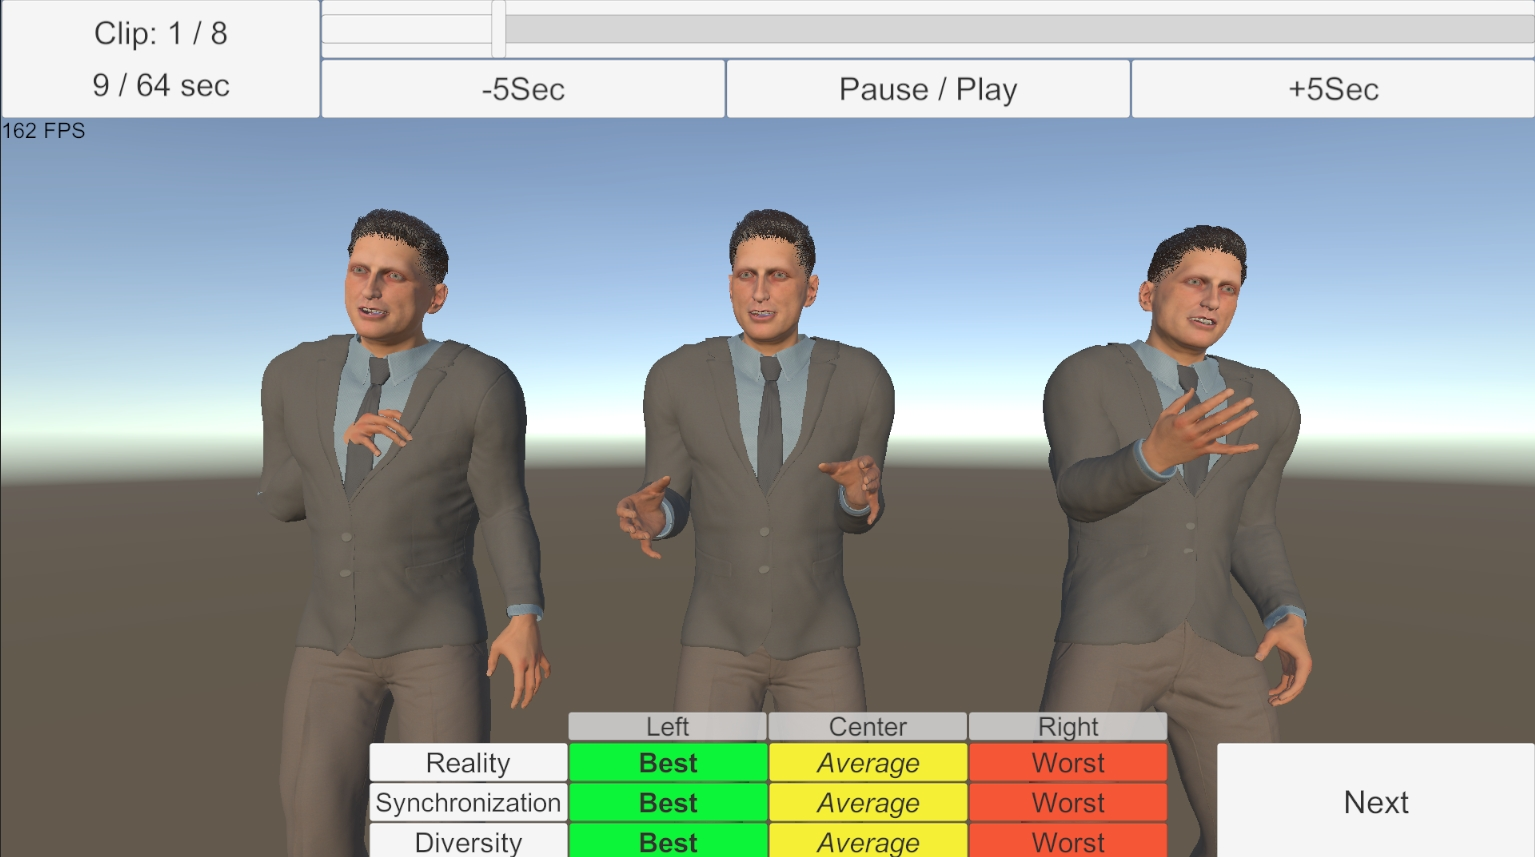
\includegraphics[width=\linewidth]{figures/UserStudyImage.png}
\caption{用户研究中使用的手势播放界面示意图。}
\label{fig:userstudy_app}
\end{figure}

% % !TEX root = ../main.tex

\chapter{Maxwell Equations}

选择二维情况,有如下的偏振矢量:
\begin{subequations}
  \begin{align}
    {\bf E} &= E_z(r, \theta) \hat{\bf z}, \\
    {\bf H} &= H_r(r, \theta) \hat{\bf r} + H_\theta(r, \theta) \hat{\bm\theta}.
  \end{align}
\end{subequations}
对上式求旋度:
\begin{subequations}
  \begin{align}
    \nabla \times {\bf E} &= \frac{1}{r} \frac{\partial E_z}{\partial\theta}
      \hat{\bf r} - \frac{\partial E_z}{\partial r} \hat{\bm\theta}, \\
    \nabla \times {\bf H} &= \left[\frac{1}{r} \frac{\partial}{\partial r}
      (r H_\theta) - \frac{1}{r} \frac{\partial H_r}{\partial\theta} \right]
      \hat{\bf z}.
  \end{align}
\end{subequations}
因为在柱坐标系下,$\overline{\overline\mu}$ 是对角的,所以 Maxwell 方程组中电场
$\bf E$ 的旋度:
\begin{subequations}
  \begin{align}
    & \nabla \times {\bf E} = \ii \omega {\bf B}, \\
    & \frac{1}{r} \frac{\partial E_z}{\partial\theta} \hat{\bf r} -
      \frac{\partial E_z}{\partial r}\hat{\bm\theta} = \ii \omega \mu_r H_r
      \hat{\bf r} + \ii \omega \mu_\theta H_\theta \hat{\bm\theta}.
  \end{align}
\end{subequations}
所以 $\bf H$ 的各个分量可以写为:
\begin{subequations}
  \begin{align}
    H_r &= \frac{1}{\ii \omega \mu_r} \frac{1}{r}
      \frac{\partial E_z}{\partial\theta}, \\
    H_\theta &= -\frac{1}{\ii \omega \mu_\theta}
      \frac{\partial E_z}{\partial r}.
  \end{align}
\end{subequations}
同样地,在柱坐标系下,$\overline{\overline\epsilon}$ 是对角的,所以 Maxwell 方程
组中磁场 $\bf H$ 的旋度:
\begin{subequations}
  \begin{align}
    & \nabla \times {\bf H} = -\ii \omega {\bf D}, \\
    & \left[\frac{1}{r} \frac{\partial}{\partial r}(r H_\theta) - \frac{1}{r}
      \frac{\partial H_r}{\partial\theta} \right] \hat{\bf z} = -\ii \omega
      {\overline{\overline\epsilon}} {\bf E} = -\ii \omega \epsilon_z E_z
      \hat{\bf z}, \\
    & \frac{1}{r} \frac{\partial}{\partial r}(r H_\theta) - \frac{1}{r}
      \frac{\partial H_r}{\partial\theta} = -\ii \omega \epsilon_z E_z.
  \end{align}
\end{subequations}
由此我们可以得到关于 $E_z$ 的波函数方程:
\begin{equation}
  \frac{1}{\mu_\theta \epsilon_z} \frac{1}{r} \frac{\partial}{\partial r}
  \left(r \frac{\partial E_z}{\partial r} \right) + \frac{1}{\mu_r \epsilon_z}
  \frac{1}{r^2} \frac{\partial^2E_z}{\partial\theta^2} +\omega^2 E_z = 0.
\end{equation}

% % !TEX root = ../main.tex

\chapter{绘制流程图}

图~\ref{fig:flow_chart} 是一张流程图示意。使用 \pkg{tikz} 环境,搭配四种预定义节
点(\verb|startstop|、\verb|process|、\verb|decision| 和 \verb|io|),可以容易地
绘制出流程图。

\begin{figure}[!htp]
  \centering
  
% 定义流程图节点
\tikzstyle{startstop} = [
  rectangle,
  rounded corners,
  minimum width=4em,
  text centered,
  inner sep=1.5ex,
  draw
]
\tikzstyle{io} = [
  trapezium,
  trapezium left angle=75,
  trapezium right angle=105,
  minimum width=4em,
  text centered,
  inner sep=1.5ex,
  draw
]
\tikzstyle{process} = [
  rectangle,
  minimum width=4em,
  text centered,
  inner sep=1.5ex,
  draw
]
\tikzstyle{decision} = [
  diamond,
  minimum width=4em,
  aspect=2,
  text centered,
  draw
]
\tikzstyle{arrow} = [-{LaTeX}]

\begin{tikzpicture}[node distance=1.5cm, every node/.style={font=\footnotesize}]
  % 设置节点
  \node[startstop] (pic) {待测图片};
  \node[io, below of=pic] (bg) {读取背景};
  \node[process, below of=bg] (pair) {匹配特征点对};
  \node[decision, below of=pair, yshift=-2ex] (threshold) {多于阈值};
  \node[decision, right of=threshold, xshift=3cm] (clear) {清晰?};
  \node[process, right of=pair, xshift=3cm] (capture) {重采};
  \node[process, below of=threshold, yshift=-2ex] (matrix_p) {透视变换矩阵};
  \node[process, right of=matrix_p, xshift=3cm] (matrix_a) {仿射变换矩阵};
  \node[process, below of=matrix_p] (reg) {图像修正};
  \node[startstop, below of=reg] (return) {配准结果};
    
  % 连接节点
  \draw[arrow] (pic) -- (bg);
  \draw[arrow] (bg) -- (pair);
  \draw[arrow] (pair) -- (threshold);

  \draw[arrow] (threshold) -- node[above] {否} (clear);

  \draw[arrow] (clear) -- node[right] {否} (capture);
  \draw[arrow] (capture) |- (pic);
  \draw[arrow] (clear) -- node[right] {是} (matrix_a);
  \draw[arrow] (matrix_a) |- (reg);

  \draw[arrow] (threshold) -- node[left] {是} (matrix_p);
  \draw[arrow] (matrix_p) -- (reg);
  \draw[arrow] (reg) -- (return);
\end{tikzpicture}

  \bicaption{绘制流程图效果}{Flow chart}
  \label{fig:flow_chart}
\end{figure}


% 结尾部分
\backmatter

% 用于盲审的论文需隐去致谢、发表论文、科研成果、简历

% 致谢
% !TEX root = ../main.tex

\begin{acknowledgements}
  感谢那位最先制作出博士学位论文 \LaTeX{} 模板的物理系同学!

  感谢 William Wang 同学对模板移植做出的贡献!

  感谢 \href{https://github.com/weijianwen}{@weijianwen} 学长开创性的工作!

  感谢 \href{https://github.com/sjtug}{@sjtug} 对 0.10 及之后版本的开发和维护工作!

  感谢所有为模板贡献过代码的\href{https://github.com/sjtug/SJTUThesis/graphs/contributors}{同学们}, 以及所有测试和使用模板的各位同学!

  感谢 \LaTeX 和 \href{https://github.com/sjtug/SJTUThesis}{SJTUThesis},帮我节省了不少时间。
\end{acknowledgements}


% 发表论文及科研成果
% 盲审论文中,发表论文及科研成果等仅以第几作者注明即可,不要出现作者或他人姓名
% !TEX root = ../main.tex

\begin{achievements}

\subsection*{学术论文}

\begin{bibliolist}{00}
  \item Chen H, Chan C~T. Acoustic cloaking in three dimensions using acoustic metamaterials[J]. Applied Physics Letters, 2007, 91:183518.
  \item Chen H, Wu B~I, Zhang B, et al. Electromagnetic Wave Interactions with a Metamaterial Cloak[J]. Physical Review Letters, 2007, 99(6):63903.
\end{bibliolist}

\begin{bibliolist*}{00}
  \item 第一作者. 中文核心期刊论文, 2007.
  \item 第一作者. EI 国际会议论文, 2006.
\end{bibliolist*}

\subsection*{专利}

\begin{bibliolist}{00}
  \item 第一发明人, “永动机”, 专利申请号202510149890.0.
\end{bibliolist}

\begin{bibliolist*}{00}
  \item 第一发明人, “永动机”, 专利申请号XXXXXXXXXXXX.X.
\end{bibliolist*}

\end{achievements}


% 简历
% !TEX root = ../main.tex

\begin{resume}
  \subsection*{基本情况}
    某某,yyyy 年 mm 月生于 xxxx。

  \subsection*{教育背景}
  \begin{itemize}
    \item yyyy 年 mm 月至今,上海交通大学,博士研究生,xx 专业
    \item yyyy 年 mm 月至 yyyy 年 mm 月,上海交通大学,硕士研究生,xx 专业
    \item yyyy 年 mm 月至 yyyy 年 mm 月,上海交通大学,本科,xx 专业
  \end{itemize}

  \subsection*{研究兴趣}
    \LaTeX{} 排版

  \subsection*{联系方式}
  \begin{itemize}
    \item 地址: 上海市闵行区东川路 800 号,200240
    \item E-mail: \email{john_smith@sjtu.edu.cn}
  \end{itemize}
\end{resume}


% 学士学位论文要求在最后有一个大摘要,单独编页码
% !TEX root = ../main.tex

\begin{digest}
  An imperial edict issued in 1896 by Emperor Guangxu, established Nanyang
  Public School in Shanghai. The normal school, school of foreign studies,
  middle school and a high school were established. Sheng Xuanhuai, the person
  responsible for proposing the idea to the emperor, became the first president
  and is regarded as the founder of the university.

  During the 1930s, the university gained a reputation of nurturing top
  engineers. After the foundation of People's Republic, some faculties were
  transferred to other universities. A significant amount of its faculty were
  sent in 1956, by the national government, to Xi'an to help build up Xi'an Jiao
  Tong University in western China. Afterwards, the school was officially
  renamed Shanghai Jiao Tong University.

  Since the reform and opening up policy in China, SJTU has taken the lead in
  management reform of institutions for higher education, regaining its vigor
  and vitality with an unprecedented momentum of growth. SJTU includes five
  beautiful campuses, Xuhui, Minhang, Luwan Qibao, and Fahua, taking up an area
  of about \qty{3225833}{\square\metre}. A number of disciplines have been
  advancing towards the top echelon internationally, and a batch of burgeoning
  branches of learning have taken an important position domestically.

  Today SJTU has 31 schools (departments), 63 undergraduate programs, 250
  masters-degree programs, 203 Ph.D. programs, 28 post-doctorate programs, and
  11 state key laboratories and national engineering research centers.

  SJTU boasts a large number of famous scientists and professors, including 35
  academics of the Academy of Sciences and Academy of Engineering, 95 accredited
  professors and chair professors of the ``Cheung Kong Scholars Program'' and
  more than \num{2000} professors and associate professors.

  Its total enrollment of students amounts to \num{35929}, of which \num{1564}
  are international students. There are \num{16802} undergraduates, and
  \num{17563} masters and Ph.D. candidates. After more than a century of
  operation, Jiao Tong University has inherited the old tradition of ``high
  starting points, solid foundation, strict requirements and extensive
  practice.'' Students from SJTU have won top prizes in various competitions,
  including ACM International Collegiate Programming Contest, International
  Mathematical Contest in Modeling and Electronics Design Contests. Famous
  alumni include Jiang Zemin, Lu Dingyi, Ding Guangen, Wang Daohan, Qian Xuesen,
  Wu Wenjun, Zou Taofen, Mao Yisheng, Cai Er, Huang Yanpei, Shao Lizi, Wang An
  and many more. More than 200 of the academics of the Chinese Academy of
  Sciences and Chinese Academy of Engineering are alumni of Jiao Tong
  University.
\end{digest}


%TC:endignore

\end{document}
